%----------------------------------------------------------
\documentclass[11pt, oneside]{book} %

\usepackage{amsmath} %
\usepackage{amsfonts} %
\usepackage{amssymb} %
\usepackage{graphicx} %
\usepackage{wrapfig} %
\usepackage{sidecap}
\usepackage{subcaption}
\usepackage{setspace}
\usepackage{algorithm}
\usepackage[noend]{algpseudocode}

%----------------------------------------------------------
\newtheorem{theorem}{Theorem}
\newtheorem{acknowledgement}[theorem]{Acknowledgement}
%\newtheorem{algorithm}[theorem]{Algorithm}
\newtheorem{axiom}[theorem]{Axiom}
\newtheorem{case}[theorem]{Case}
\newtheorem{claim}[theorem]{Claim}
\newtheorem{conclusion}[theorem]{Conclusion}
\newtheorem{condition}[theorem]{Condition}
\newtheorem{conjecture}[theorem]{Conjecture}
\newtheorem{corollary}[theorem]{Corollary}
\newtheorem{criterion}[theorem]{Criterion}
\newtheorem{definition}[theorem]{Definition}
\newtheorem{example}[theorem]{Example}
\newtheorem{exercise}[theorem]{Exercise}
\newtheorem{lemma}[theorem]{Lemma}
\newtheorem{notation}[theorem]{Notation}
\newtheorem{problem}[theorem]{Problem}
\newtheorem{proposition}[theorem]{Proposition}
\newtheorem{remark}[theorem]{Remark}
\newtheorem{solution}[theorem]{Solution}
\newtheorem{summary}[theorem]{Summary} 
\newenvironment{proof}[1][Proof]{\textbf{#1.} }{\ \rule{0.5em}{0.5em}}
%----------------------------------------------------------

\usepackage{hyperref}
\onehalfspacing
%----------------------------------------------------------
\begin{document}

% First Page.
\frontmatter
\title{Proyecto de Fin de Carrera. \\ Desarrollo e Implementación de algoritmo de seguimiento para Vehículos Aeréos no Tripulados}
\author{Pablo Ram\'on Soria}
\date{2014-09-15}
\maketitle

%----------------------------------------------------------
% Table of contenst
\tableofcontents

%----------------------------------------------------------
% Preface
\chapter{Prefacio}
This project is the result of half-year research at the Group of Robotics, Vision and Control at the School of Engineering of the University of Seville. \\

%% 666 TODO: Cosas que han pasado desarrollando

My first word of thanks goes to Bego\~na C. Arrue Ull\'es for helping me not only defining my research question, but also giving me the opportunity to work as an intern inside the GRVC. \\

A Second word of thanks goes to my parents for their motivational support, although I was absent during this time due to studies and works.  \\

Thirdly, I want to thank my colleague who motivate me to always improve my code and not to settle for the basics.  \\



%----------------------------------------------------------
% Chapter 1. Introduction
\chapter{Introducci\'on}
\section{Objetivos}

El principal objetivo de este documento es describir el algoritmo de seguimiento para vigilancia para ordenadores de abordo de UAVs \cite{Image_processing_UAV}. Este proyecto se forma parte de un proyecto Europeo, cuyo prop\'osito es mejorar la seguridad y fiabilidad de los programas de vehículos no tripulados.

 
%Firstly, previously to talk about those results, there's an explanation of each fragment of the algorithm and their equations. \\
%The following chapter, is about the first implementation inside a simulator. The program of the ground station would be the same as the real, but quadcopters and cameras are simulated with V-REP software. \\
%Finally, on the last chapter, the application will be tested inside the embedded computers "Odroid u3" in order to get as much information as possible about speediness of the  algorithm and errors on estimations.

\section{Estado del Arte}
Computer vision entails mining information from images and video to extract meaningful information. We encounter state-of-the-art computer vision techniques every day-surveillance camera systems \cite{traffic_surveillance_pergamon} \cite{distributed_surveillance} \cite{vehicle_detection}, face detection in our digital cameras, sports analysis, and the recent very popular Kinect system by Microsoft \cite{Kinect_intro}, to name a few. In all of these situations, computer algorithms process images and video to get useful information, so that a human user need not look through, say, hours and hours of surveillance footage. Computer vision research has come a long way over the decades, and today you can take a picture of an object on your cellphone camera and search for it, without typing a word. \\

Particularly, we are focused on improving the computer vision algorithm together with a position estimator for surveillance operations. Task distribution \cite{Coop_Surv_aerial_JJ} \cite{Consensus_reaching_Xiao} \cite{Adaptative_tast_Meuth} \cite{distributed_architecture_Ivan_Maza}  is a key issue in surveillance, many approaches were based on reducing the size and the requirements of the UAVs but increasing the number of these ones. That allows to the system to simplify the tasks and reduce the areas of every vehicle. The Decentralized of the task \cite{descentralized_task_UAV} (That has the associated increasing of the number of the watchers) results in the need of a network that allows to every device to communicate each other and share their information. \\

In regard to the vision algorithm, there are many different method to extract information from every frame. These can be focused in shape segmentation and recognition \cite{shape_using_shape_context} \cite{Vehicle_recog_markov}, color segmentation \cite{} among others, including a combination of them \cite{realtime_signal_recon_shape_color} \cite{signal_recogn_shape_color} \cite{Robust_RT_tracking_color_face_Darrell}.


% 666 TODO....
%% Started the main Content
\mainmatter

%----------------------------------------------------------
% Chapter 2. Algorithmcs & Software architecture
\chapter{Algoritmia y Arquitectura de Software}
\section{Introducci\'on}
Existen muchas aproximaciones para sistemas de visi\'on basados en la segmentaci\'on \cite{fast_segmentation_Mitra} \cite{fuzzy_segmentation}. Aquellos centrados en el procesamiento a tiempo real pueden llevarse a cabo por hardware, sin embargo esto requiere una dependencia con la plataforma. En el caso de este proyecto, desarrollamos un algoritmo \'unicamente en software pudiendo aplicarse a cualquier plataforma. En rasgos generales, el software se compone de tres partes: Una primera que se encarga de la segmentación en color de la imagen y la extracción de objetos 2-D basado en el algoritmo de CMU \cite{JamesBruce_CMU_SEG} (Color Cluster Segmentation: \textbf{CCS} en adelante); Una segunda parte que recibe los objetos 2-D anteriores (y en caso de vision est\'ereo hace el emparejamiento entre ambos objetos); Y final mente un filtro de Kalman extendido \cite{GabrielTerejanu_EKF} (\textbf{EKF}) que se encarga de triangular y filtrar la posición de los objetos. 

Antes de la explicaci\'on detallada, se muestra el siguiente pseudo codigo del proceso:

\begin{algorithm}[hp]
\caption{Tracking algorithm}\label{algorithm_pseudo}
	\begin{algorithmic}[1]
	\Procedure{MainProcess}{}
		\State \Call{setUpEKF}{$params$}
		\State \Call{open}{$camera$}
		\State $\textit{img}  \gets$ \Call{GetImage}{$camera$}
		\If{$\textit{img}$ is empty} 
			\State \Return false
		\EndIf
		
		\State $\textit{objects} \gets$ \Call{Segmentation}{$img$}
		\If{size of $\textit{objects}$} 
			\State \Return false;
		\EndIf
		
		\State $\textit{state} \gets$ \Call{Tracking}{$objects$}
	\EndProcedure
	
	% --------------------------------------------------------------------------
	\Procedure{GetImage}{$VideoSource$}
		\If{$VideoSource$ is open}
			\State $image \gets VideoSource$
			\Return $image$
		\Else $\;$
			\State \Return $Null$
		\EndIf
		
	\EndProcedure
	
	% --------------------------------------------------------------------------	
	\Procedure{Segmentation}{$Image$}
		\If{$Image$ is not HSV}
			\State \Call{convertToHSV}{$Image$}
		\EndIf
		\ForAll{$pixel$ in $Image$}
			\State $pixel \gets$ \Call{conversion}{$pixel$}
		\EndFor
			\State \Return \Call{gatherObjects}{$Image$}
	\EndProcedure
	
	% --------------------------------------------------------------------------		
	\Procedure{Tracking}{$Object$}
		\State $matchedObj \gets$ \Call{Matching}{$Objects$} 
		\If{$matchedObj$ is empty}
			\State \Return $Null$
		\EndIf
		\State $state \gets$ \Call{stepEKF}{matchedObj}
		\State \Return $state$
	\EndProcedure
	
	% --------------------------------------------------------------------------	
	\end{algorithmic}
\end{algorithm}

\section{Algoritmo de Segmentaci\'on}
%----------------------------------------------------------
\subsection{Espacio de Colores}
Para extraer los objetos de la escena, el algoritmo simplifica los colores de cada imagen y agrupa los p\'ixeles en cl\'usteres de colores. \\

RGB es el espacio de colores mas com\'un, este est\'a compuesto de tres canales (Rojo, verde y azul).Sin embargo, el principal problema de este espacio de colores es que la información sobre la "pigmentaci\'on" se encuentra en los tres canales.\\

Para solventar ese problema, se usa en este proyecto el espacio de colores HSV (Hue, Saturation and Value). En este, la información sobre el color se encuentra en un único canal, por lo que es menos sensible a los cambios y las limitaciones entre un color y otro son planos en vez de superficies. \\

% HSV vs RGB figure
\begin{figure}[h]
	\centering
	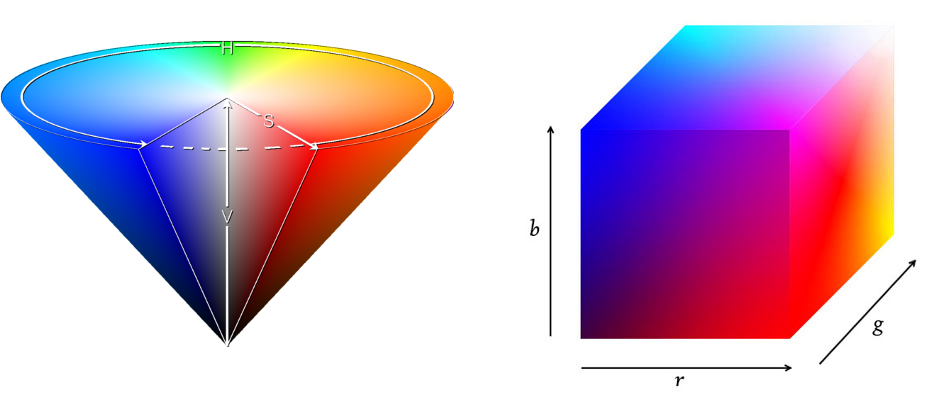
\includegraphics[width=0.75\textwidth,natwidth=944,natheight=400]{../Images/c2/HSV_vs_RGB.png}
	\caption{Espacios de colores HSV y RGB}
	\label{fig:HSV_vs_RGB}
\end{figure}

%----------------------------------------------------------
\subsection{Transformaci\'on de pixeles}
En este apartado se describe c\'omo es transformado cada p\'ixel para pasar del color inicial a uno de los colores de los cl\'usteres. Esto se lleva a cabo aplicando una serie de límites a los canales del espacio de colores \\

\begin{figure}[h]
	\centering
	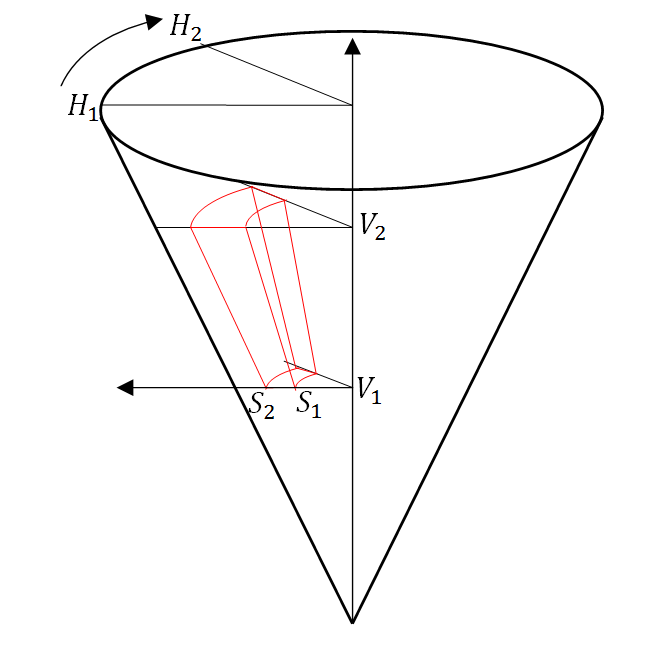
\includegraphics[width=0.5\textwidth,natwidth=659,natheight=659]{../Images/c2/DividingSubSpace.png}
	\caption{Divisi\'on del espacio de color HSV}
	\label{fig:DividingSubSpace}
\end{figure}

Una de las claves para la disminución del tiempo de computaci\'on del algoritmo es la sustitución de las condiciones $if...else...$ por in-direccionamientos de memoria y comparaciones $bitwise$. Estas son mucho m\'as r\'apidas y eficientes \cite{JamesBruce_CMU_SEG}. \\

\begin{equation}
\begin{split}
pixel\_col = H\_Range[h] \& \\
S\_Range[s] \& \\
V\_Range[v] 
\end{split}
\end{equation}
	

Para mostrar el proceso, consideramos el siguiente ejemplo. Si dividimos cada canal del espacio en diez bloques $(n_H = 10, n_S = 10$ y $n_V = 10)$ podemos definir de la siguiente forma (Indicando 1 cuando el negro pertenece a ese rango y 0 si no pertenece a ese rango)

{\centering
\[HRange[10] = \{1, 1, 1, 1, 1, 1, 1, 1, 1, 1\}\]
\[SRange[10] = \{1, 1, 1, 1, 1, 1, 1, 1, 1, 1\}\]
\[VRange[10] = \{1, 1, 1, 0, 0, 0, 0, 0, 0, 0\}\]
} 

Para comprobar si el siguiente color de p\'ixel:  $(3, 5, 1)$, pertenece al negro solo hay que evaluar la siguiente expresi\'on:

\[ pixel\_col = HRange[3] \& SRange[5] \& VRange[1] = 1 \& 1 \& 1 = 1 \]


El siguiente punto importante es que esto permite evaluar la pertenencia a muchas clases de colores de forma simultánea. Si definimos por ejemplo el azul como lo siguiente:

{\centering
\[HRange[10] = \{0, 0, 0, 0, 1, 1, 1, 0, 0, 0\}\]
\[SRange[10] = \{0, 0, 0, 0, 1, 1, 1, 1, 1, 1\}\]
\[VRange[10] = \{0, 0, 0, 1, 1, 1, 1, 1, 1, 1\}\]
}

Podremos agrupar ambos tipos así:

{\centering
\[HRange[10] = \{01, 01, 01, 01, 11, 11, 11, 01, 01, 01\}\]
\[SRange[10] = \{01, 01, 01, 01, 11, 11, 11, 11, 11, 11\}\]
\[VRange[10] = \{01, 01, 01, 10, 10, 10, 10, 10, 10, 10\}\] 
} 

Gracias a que la operaci\'on bitwise se realiza bit a bit, el color $(3,5,1)$ se puede evaluar como: 

\[pixel\_col = HRange[3] \& SRange[5] \& VRange[1] = 01 \& 11 \& 01 = 01\]

Resultando que pertenece al color negro.

En particular, en el algoritmo usamos arrays de bytes de tamaño 36, lo que significa que diferenciamos 8 colores con una resoluci\'on de $1/36$. \\

Las siguientes imágenes muestran el resultado del algoritmo con la conocida imagen \textit{Head Scene}  de la universidad de Tsukuba \ref{fig:head_scene_tsukuba_ori} \ref{fig:head_scene_tsukuba_seg}. \\


\begin{figure}[hbp]
	\centering
	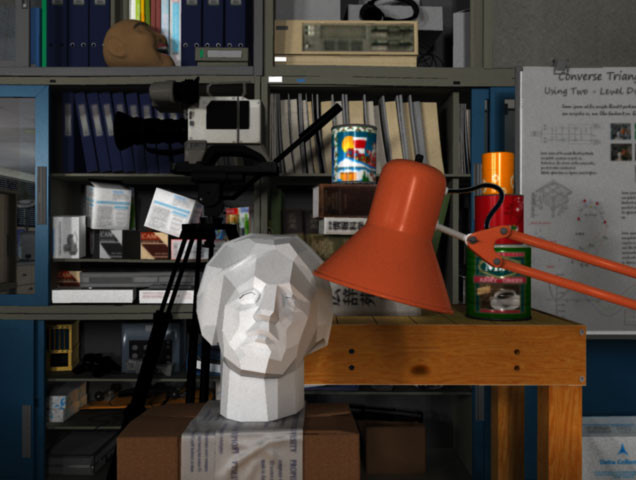
\includegraphics[width=0.4\linewidth]{../Images/c2/head_scene_tsukuba_ori}
	\caption{Imagen original de $Head Scene$}
	\label{fig:head_scene_tsukuba_ori}
\end{figure}

\begin{figure}[htp]
	\centering
	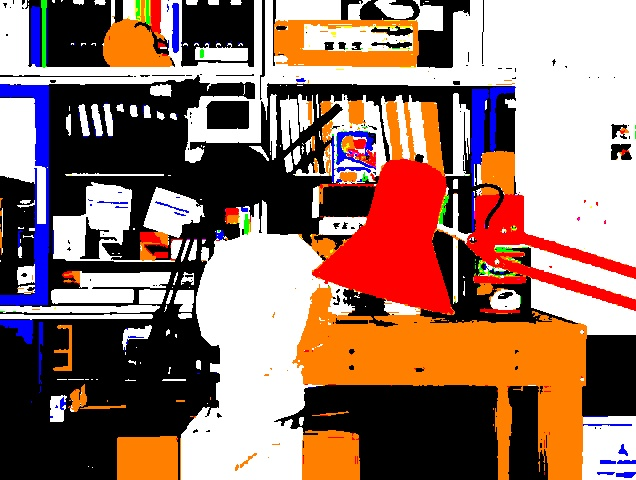
\includegraphics[width=0.4\linewidth]{../Images/c2/head_scene_tsukuba_seg}
	\caption{Imagen segmentada de $Head Scene$}
	\label{fig:head_scene_tsukuba_seg}
\end{figure}



%\begin{figure}[h]
%	\centering
%	\begin{subfigure}{0.47\linewidth}
%		\centering
%		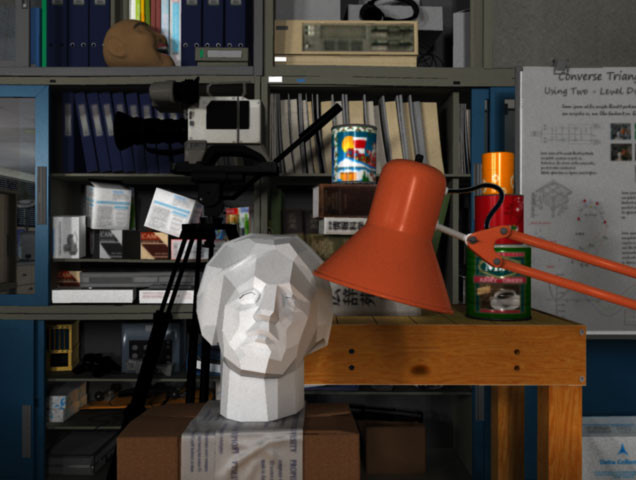
\includegraphics[width=\linewidth]{../Images/c2/head_scene_tsukuba_ori}
%		\caption{Original image of the Head Scene}
%		\label{fig:head_scene_tsukuba_ori}
%	\end{subfigure}
%	~
%	\begin{subfigure}{0.47\linewidth}
%		\centering
%		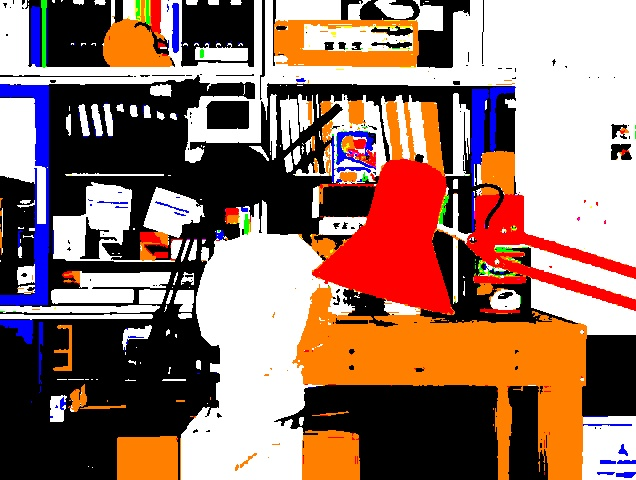
\includegraphics[width=\linewidth]{../Images/c2/head_scene_tsukuba_seg}
%		\caption{Segmented image of the Head Scene}
%		\label{fig:head_scene_tsukuba_seg}
%	\end{subfigure}
%	\caption{Head Scene, University of Tsukuba}
%	\label{fig:Head_Scene}
%\end{figure}



%----------------------------------------------------------
\subsection{Run-length encoding}
La compresi\'on RLE o $Run-length encoding$ es un m\'etodo simple de compresión de datos donde cada tira de datos del mismo tipo es comprimida por una pareja de $valor$ y $cantidad$. Por ejemplo, la siguiente $tira$: \\

\textit{WWWWWWWBBBBBBBBBCCCCCCWWWWWWWWWWWWWWWW} \\

Codificada seria la siguiente: \\
\textit{W7B9C6W16}

En este documento RLE se usa para reducir el tama\~no de la imagen, permitiendo iterar r\'apidamente en cada iteraci\'n. \\

Este tipo de compresión es muy útil en las imágenes que tienen colores homogéneos, sin embargo puede aumentar el tama\~no de la misma si los p\'ixeles tienen demasiado ruido: \\

\begin{enumerate}
	\item Homog\'eneo: \textit{WWWWWWWWWWWWWWWWWWWW $\Rightarrow$ W20} \\
	\item Heterog\'eneo: \textit{WAWAWAWAWA $\Rightarrow$ W1A1W1A1W1A1W1A1} \\
\end{enumerate}

%----------------------------------------------------------
\subsection{Agrupaci\'on de p\'ixeles. Creaci\'on del objeto}

Once every row of the picture is encoded with RLE it's necessary to connect the regions to extract information about the objects \ref{fig:RLE1}. This is made in two phases. The first one seek per line the adjacent runs with the same color and connect them \ref{fig:RLE2}. Once every line was explored \ref{fig:RLE3}, the second phase look for objects that are splitted due to the first clustering \ref{fig:RLE4}. During the last phase every info is stored in an $"object class"$ that store the size (in pixels), the bouncing box and its centroid.

\begin{figure}
	\centering
	\begin{subfigure}{\linewidth}
		\centering
		\begin{subfigure}{0.4\linewidth}
			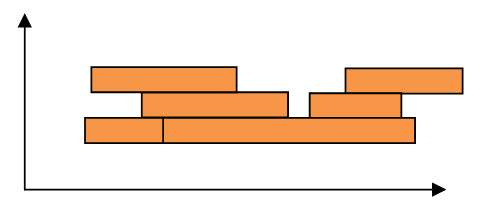
\includegraphics[width=\linewidth]{../Images/c2/RLE1}
			\caption{Runs are disjointed}
			\label{fig:RLE1}
		\end{subfigure}
		%--------------------------------------------------------------------
		\begin{subfigure}{0.4\linewidth}
			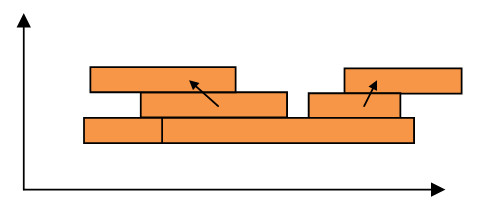
\includegraphics[width=\linewidth]{../Images/c2/RLE2}
			\caption{Vertical scanning result in neighbors clustering}
			\label{fig:RLE2}
		\end{subfigure}
	\end{subfigure}
	~
	\begin{subfigure}{\linewidth}
		\centering
   		\begin{subfigure}{0.4\linewidth}
   			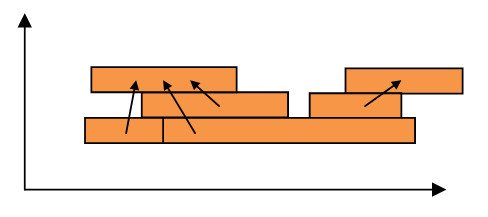
\includegraphics[width=\linewidth]{../Images/c2/RLE3}
   			\caption{All lines joined}
   			\label{fig:RLE3}
   		\end{subfigure}
   		%--------------------------------------------------------------------
   		\begin{subfigure}{0.4\linewidth}
   			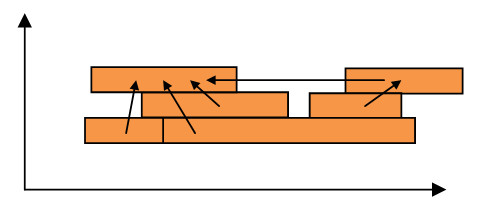
\includegraphics[width=\linewidth]{../Images/c2/RLE4}
   			\caption{Last scanning looking for splitted objects}
   			\label{fig:RLE4}
   		\end{subfigure}
	\end{subfigure}
	\caption{Object creation  from RLEs}
\end{figure}


\section{Filtro de Kalman Extendido}
%----------------------------------------------------------
\subsection{Modelo del sistema} \label{subsec:system_model}
El sistema consiste en un quadrotor portando una c\'amara. Las coordenadas de los puntos del espacio respecto a los ejes del la c\'amara son:

\begin{equation}
\left. \overrightarrow{P_{obj}} = \overrightarrow{C} + \bar{\bar{R}}^{T}*\overrightarrow{P_{c}} \right|_c
\end{equation}

\begin{equation} \label{eq:system_equation}
P_{obj} = 
	\left.
	\begin{pmatrix}
	x \\
	y \\
	z \\
	\end{pmatrix}
=
	\begin{pmatrix}
	c_x \\
	c_y \\
	c_z \\
	\end{pmatrix}
+
	\begin{pmatrix}
	r_{11} & r_{21} & r_{31} \\
	r_{12} & r_{22} & r_{32} \\
	r_{13} & r_{23} & r_{33} \\
	\end{pmatrix}
*
	\begin{pmatrix}
	x_c \\
	y_c \\
	z_c \\
	\end{pmatrix}
	\right|_c
\end{equation}


%----------------------------------------------------------
\subsection{Camera Model}
	El modelo de la c\'amara \cite{camera_models}  y sus ecuaciones fueron descritas en la secci\'on del algoritmo de matching.
	
	\begin{figure}[ph]
		\centering
		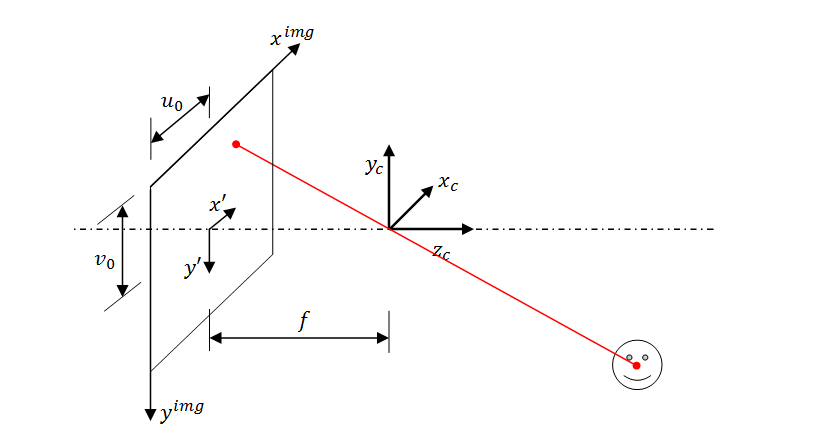
\includegraphics[width=0.7\linewidth]{../Images/c2/pinhole_model}
		\caption{}
		\label{fig:pinhole_model}
	\end{figure}

	
%----------------------------------------------------------
\subsection{Extended Kalman Filter}

El filtro de Kalman es un algoritmo iterativo de estimaci\'on de estados de sistemas din\'amicos. Este suele ser aplicado cuando se necesita saber el estado de un sistema con m\'as mediciones que grados de libertad del sistema y para la atenuaci\'on de ruido blanco en las estimaciones. En este caso usamos una aproximaci\'on lineal del sistema con una variante llamada Filtro de Kalman Extendido \cite{GabrielTerejanu_EKF} (o EKF).

Sea el sistema a estudiar:

\begin{gather}
x_k = f(x_{k-1}) + w_{k-1} \\
z_k = h(x_k) + v_k
\end{gather}

Cada paso del EKF esta formado de dos iteraciones llamadas "Predictor" y "corrector"

\begin{itemize}
   \item Predictor Step
		\begin{gather}
			x_k^{f} \approx f(x_{k-1}^{a}) \\
			P_k^{f} = J_f(x_{k-1}^{a}) P_{k-1} J_f^{T}(x_{k-1}^{a}) + Q_{k-1}
		\end{gather}

	\item Corrector Step
		\begin{gather}
			P_k = (I - K_k J_h(x_k^{f}))P_k^{f} \\
			K_k = P_k^{f} J^{T}_h(x_k^{f}) (J_h(x_k^{f}) P_k^{f} J_h^{T}(x_k ^{f}) + R_k)^{-1} \\
			x_k^{a} \approx x_k^{f} + K_k (z_k - h(x_k^{f}))
		\end{gather}
\end{itemize}

\section{Arquitectura General} \label{sec:SoftArch}
La siguiente figura \ref{fig:System_Architecture} ejemplifica la arquitectura del sistema y de que se compone: \\
% System architecture image
\begin{figure}[th]
	\centering
	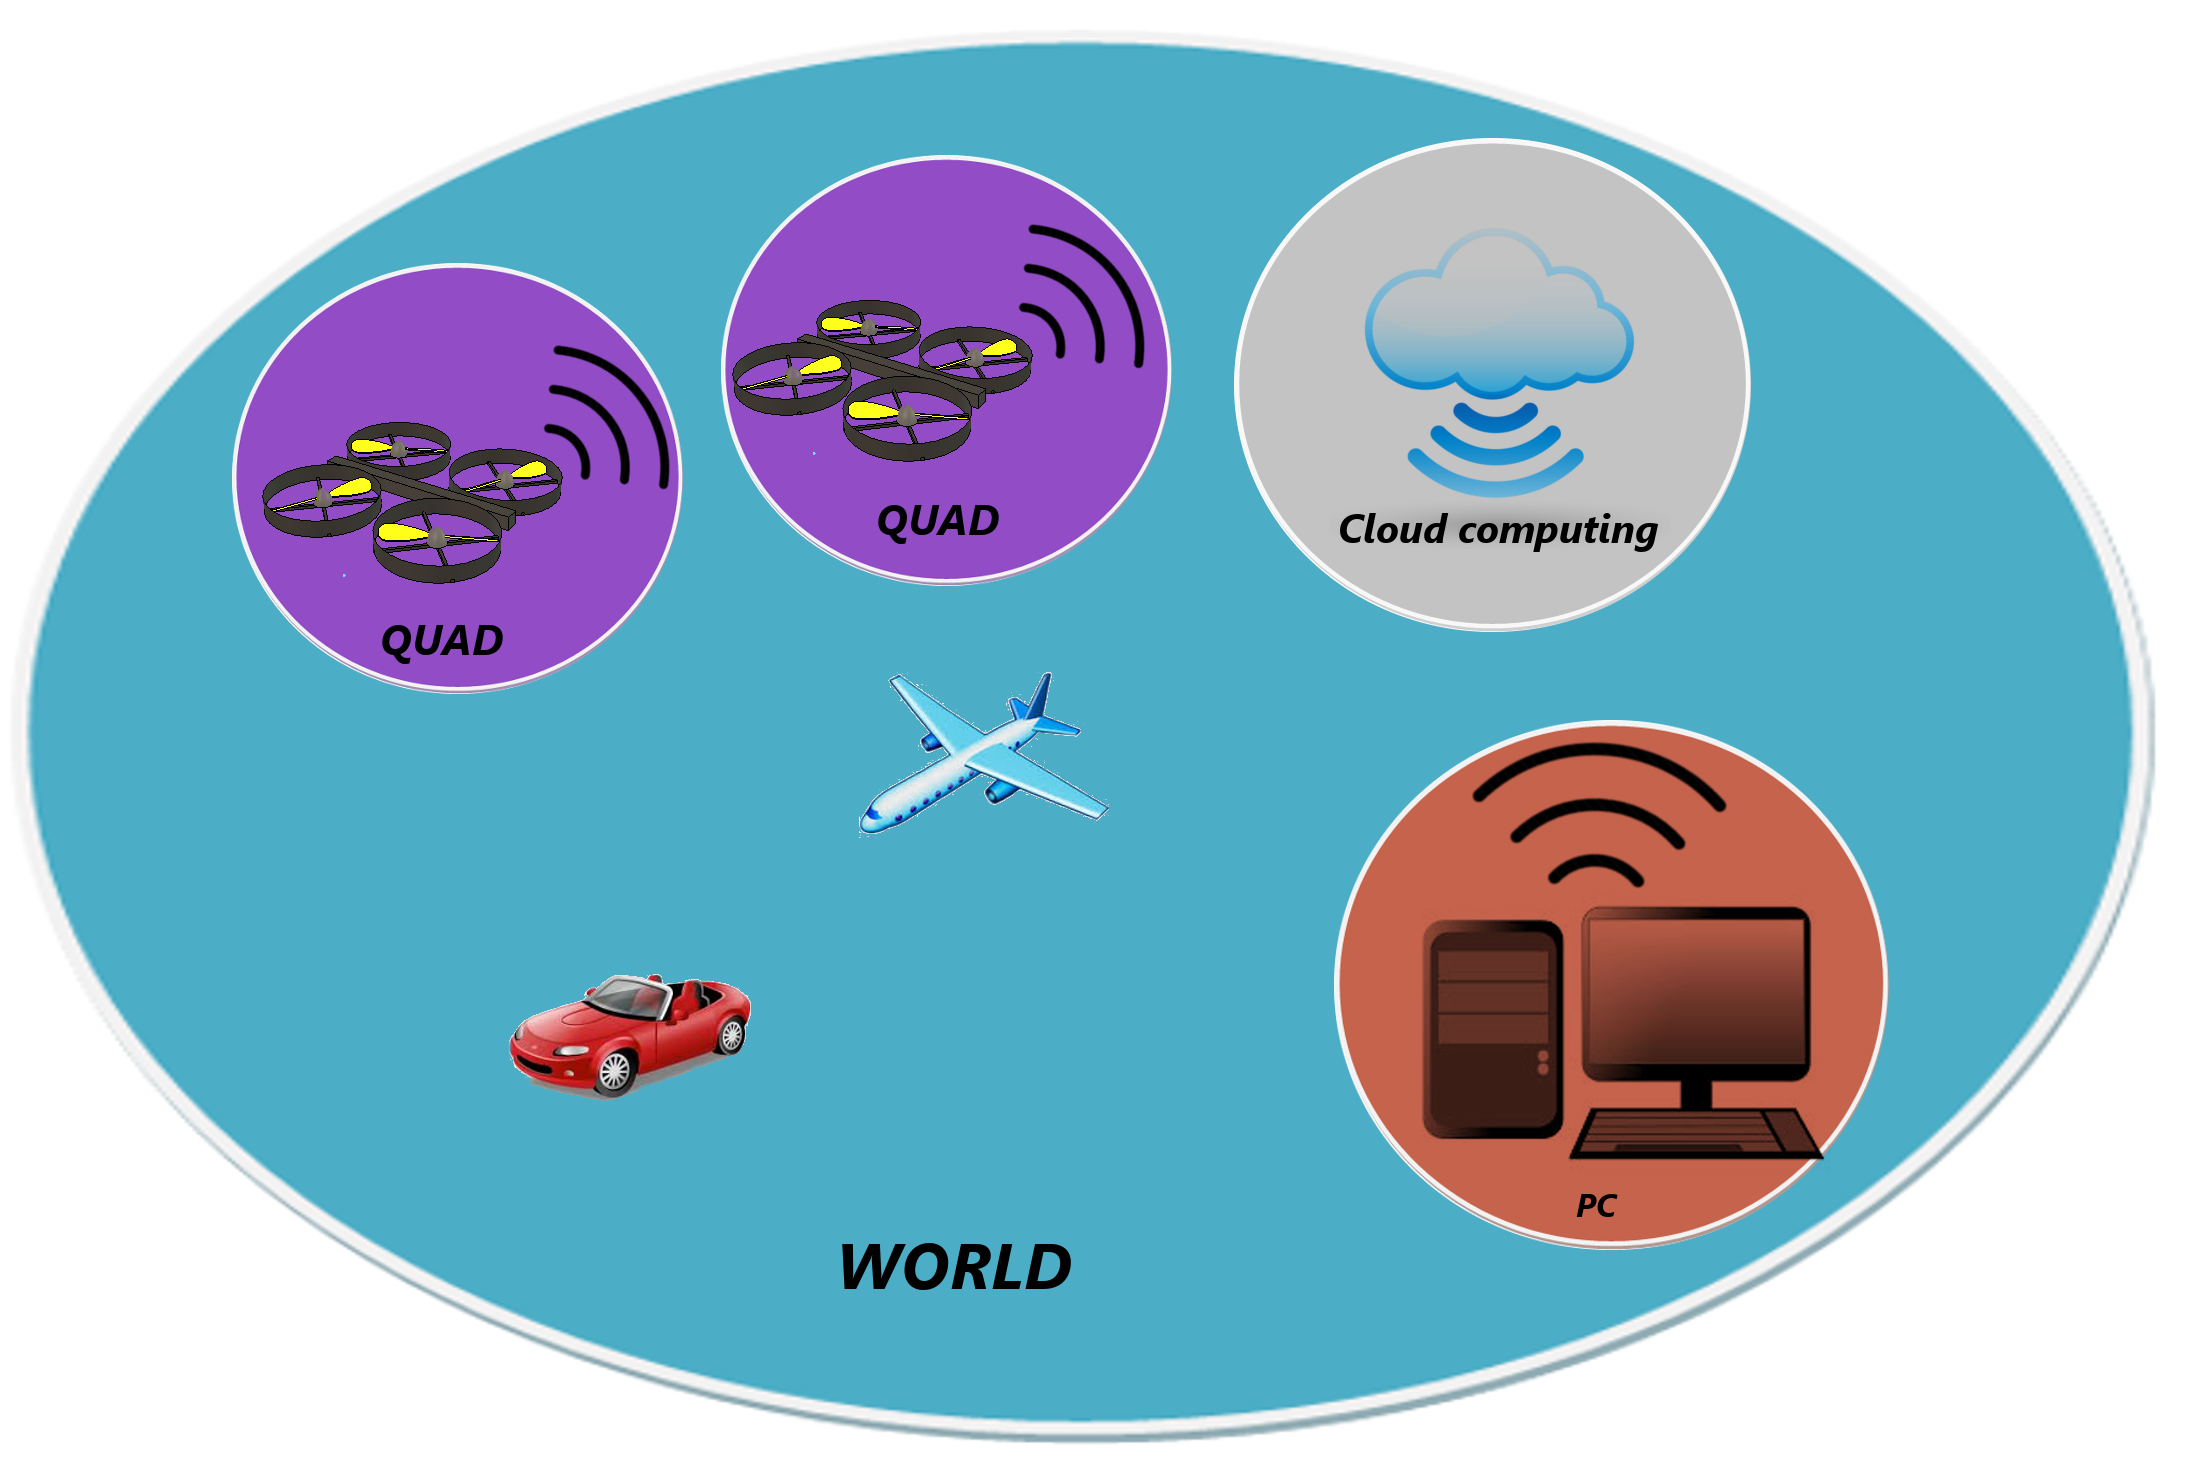
\includegraphics[width=0.50\textwidth,natwidth=220,natheight=1467]{../Images/c2/Architecture.png}
	\caption{Arquitectura del sistema}
	\label{fig:System_Architecture}
\end{figure}


\begin{itemize}
  \item Conjunto de Quadrotores.
  \item Estaci\'on de tierra.
  \item "$La Nube$".
  \item Objetivos.
\end{itemize}

Cada quadrotor consta de una c\'amara y un ordenador de abordo que ejecuta el algoritmo, la informaci\'on obtenida se manda a la estaci\'on en tierra que la procesa y ejecuta el algoritmo de seguimiento.

\newpage
\subsection{Quadrotors Software}

	\begin{figure}[hp]
		\begin{center}
			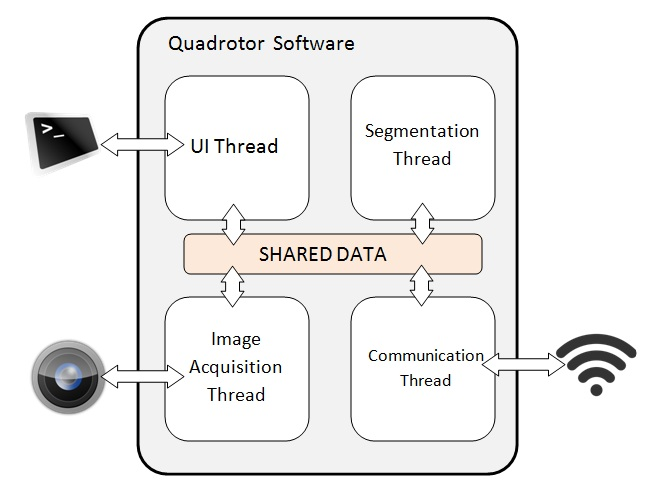
\includegraphics[width=0.7\linewidth]{../Images/c2/Quadsoftware}
		\end{center}
		\caption{Quadrotor's Software}
		\label{fig:Quadsoftware}
	\end{figure}

	La figura \ref{fig:Quadsoftware} muestra esquematicamente la estructura del software de cada quadrotor que se compone de varios threads para paralelizar el algoritmo:
	
	
	\begin{itemize}
		\label{itemize:quadappthreads}
		\item Thread de interfaz de usuario.
		\item Thread de adquisici\'on de im\'agenes.
		\item Thread de segmentaci\'on de im\'agenes.
		\item Thread de comunicaci\'on.
	\end{itemize}
	
\subsection{Software de la estaci\'on de tierra}
	\begin{figure}[th]
		\begin{center}
			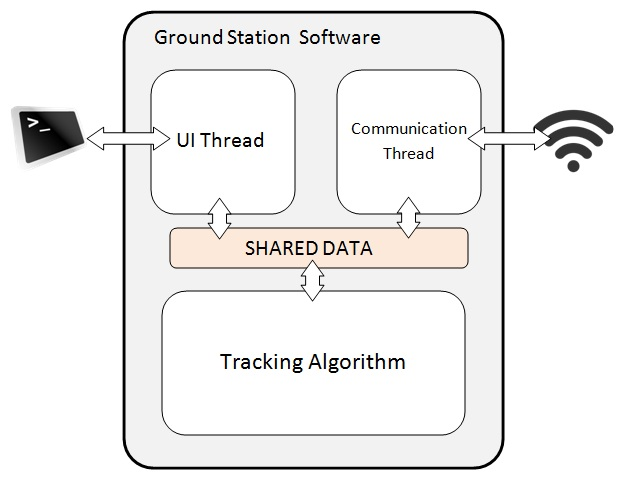
\includegraphics[width=0.7\linewidth]{../Images/c2/GroundStationsoftware}
		\end{center}
		\caption{Ground station's Software}
		\label{fig:GroundStation}
	\end{figure}

	\begin{itemize}
		\item Thread de interfaz de usuario.
		\item Thread de comunicaci\'on.
		\item Thread de algoritmo de seguimiento.
	\end{itemize}

	
\subsection{Conclusion}
La funcionalidad de ambos, quadrotor y estaci\'on de tierra puede ser modificada facilmente añadiendo threads a la ejecuci\'on del programa. Adem\'as gracias a las capas de abstracci\'on cada parte de la estructura puede ser remplazada por otra que la mejore o para adaptar el sistema por ejemplo:

\begin{itemize}
  \item Conjunto de quadrotores $\Longrightarrow$ UGVs y UAVs variados.
  \item Estaci\'on de tierra $\Longrightarrow$ M\'ultiples estaciones de tierra ($Cloud computation$ \cite{Cloud_computing} o estaciones m\'oviles)
  \item Punto de acceso $\Longrightarrow$  M\'odulos GSM ($Cloud computation$ \ref{cloud_computing})
  \item Objetivos.
\end{itemize}


% 666 TODO: terminar


%----------------------------------------------------------
% Chapter 3. Simulation on VREP 
\chapter{Simulaci\'on en VREP}
\section{Introducci\'on}
The robot simulator V-REP, with integrated development environment, is based on a distributed control architecture: each object/model can be individually controlled via an embedded script, a plugin, a ROS node, a remote API client, or a custom solution. This makes V-REP very versatile and ideal for multi-robot applications. Controllers can be written in C/C++, Python, Java, Lua, Matlab, Octave or Urbi. \\

Previous to real implementation, in order to probe the effectiveness of the vision algorithm and the complete tracking architecture, the situation was simulated in this program. In this chapter will be described the process and the results of this simulations.

\subsection{The GUI}

In the following picture (Picture: \ref{fig:VREP_GUI}) shows the common user's interface of the simulator. At the top, there is the common edit buttons and camera movement through the scene. Also at the top on the right are the basic simulate configuration and buttons.

Some pre-created objects can be found in the model browser menu. There are a huge variety of mobile and fixed robots with their own AI and behavior integrated. This acts can be modified or amplified adding plugins or scripts as described previously.

Finally in the center of the interface the interface is the scene visualization. Objects are organized in the hierarchy menu on the left side of the scene.

\begin{figure}
	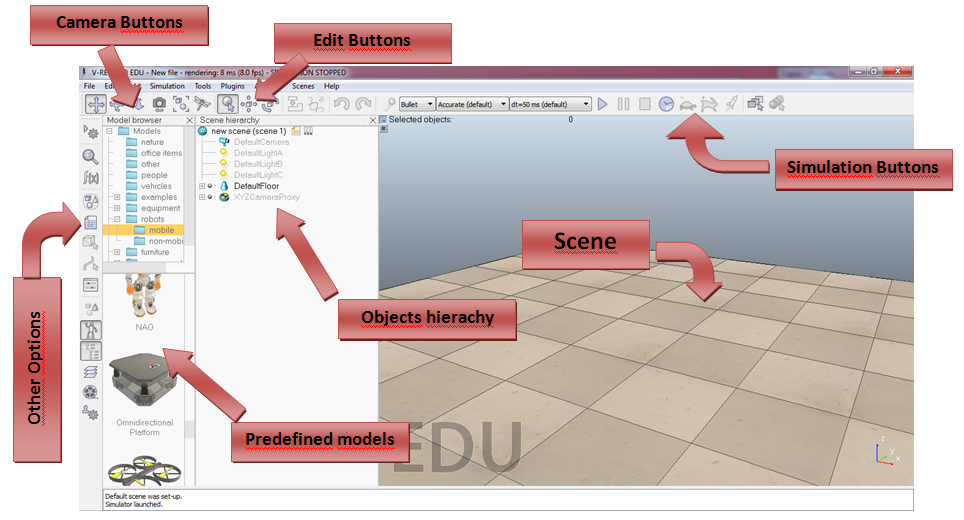
\includegraphics[width=\textwidth,natwidth=964,natheight=520]{../Images/c3/vrep_main.png}
	\caption{V-REP GUI}
	\label{fig:VREP_GUI}
\end{figure}




\section{Implementaci\'on en VREP}
%-------------------------------------------------------------------------------------------------------
%-------------------------------------------------------------------------------------------------------
%-------------------------------------------------------------------------------------------------------
\subsection{Introducci\'on a la secci\'on}
Cada apartado es una simulaci\'on de la futura aplicaci\'on del algoritmo. Cada una consta de una escena propia mostrada como en la figura \ref{fig:VREP_scene_example}. El resultado se visualiza por consola en el formato que muestra la figura \ref{fig:Ground_Tracking_VREP_Console}. \\

\begin{figure}[ht]
	\centering
	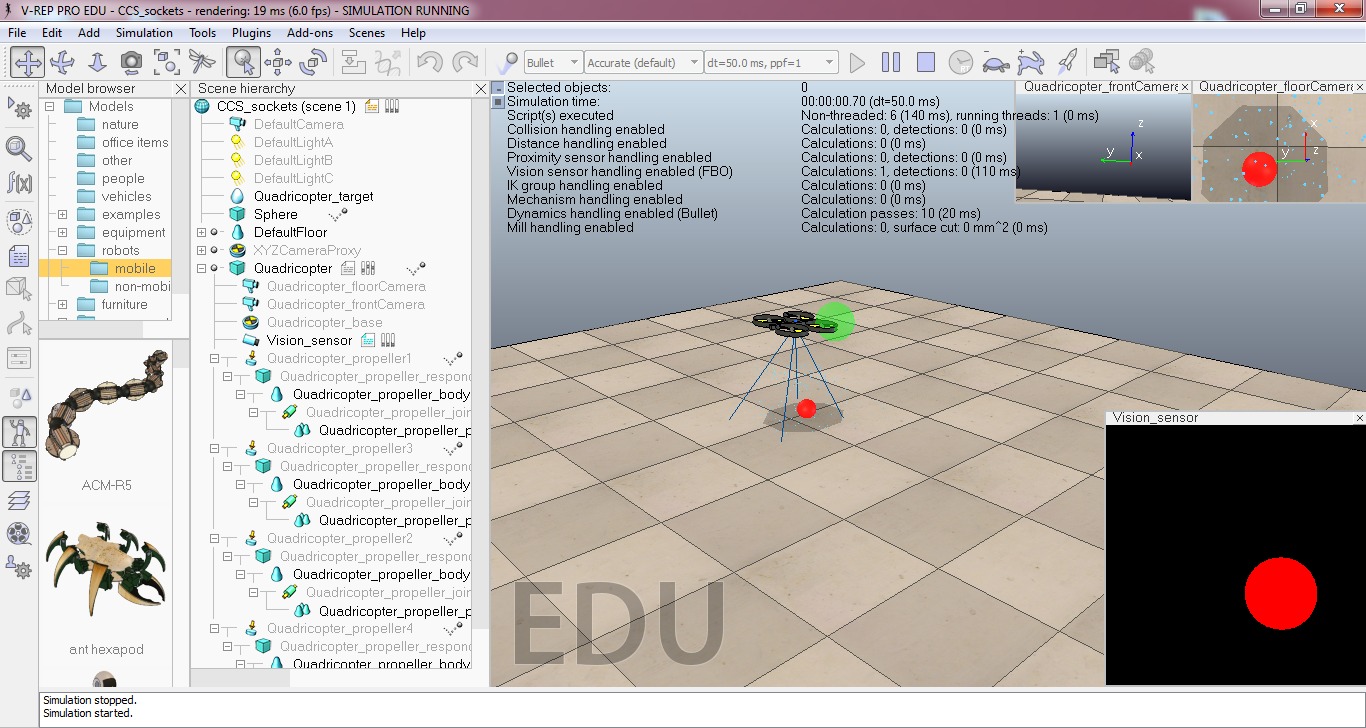
\includegraphics[width=0.8\textwidth,natwidth=1366,natheight=728]{../Images/c3/ground_tracking_scene.png}
	\caption{Ground Tracking Scene}
	\label{fig:VREP_scene_example}
\end{figure}

\begin{figure}[ht]
	\centering
	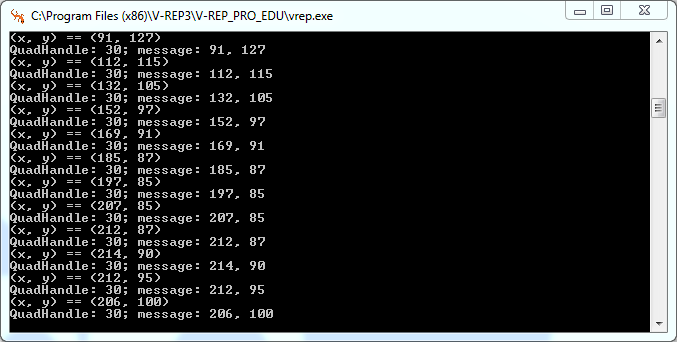
\includegraphics[width=0.8\textwidth,natwidth=677,natheight=342]{../Images/c3/ground_tracking_vrep_console.png}
	\caption{Ground Tracking V-REP Console}
	\label{fig:Ground_Tracking_VREP_Console}
\end{figure}

La estación en tierra se simula con una aplicaci\'on en el mismo ordenador que ejecuta la simualaci\'on tal que los resultados se muestran tambi\'en por consola del siguiente modo: \ref{fig:Ground_Tracking_Server_Console}.

\begin{figure}[ht]
	\centering
	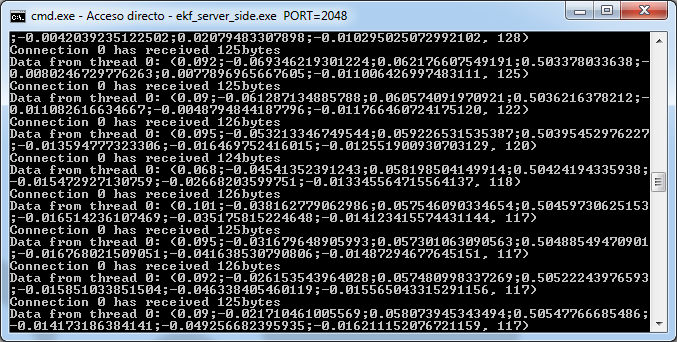
\includegraphics[width=0.8\textwidth,natwidth=677,natheight=342]{../Images/c3/ground_tracking_server_console.png}
	\caption{Ground Tracking Server Console}
	\label{fig:Ground_Tracking_Server_Console}
\end{figure}

Ambos procesos (Quadrotor y estaci\'on de tierra) generan unos ficheros de LOG que se usar\'an para analizar los resultados.

%-------------------------------------------------------------------------------------------------------
%-------------------------------------------------------------------------------------------------------
%-------------------------------------------------------------------------------------------------------
%-------------------------------------------------------------------------------------------------------
%-------------------------------------------------------------------------------------------------------
%-------------------------------------------------------------------------------------------------------
\subsection{Ejemplo de resultados - Seguimiento en tierra de m\'ultiples objetivos}
\subsubsection{Preparaci\'on}
 Este experimento consta de un solo quadrotor y dos obetivos \ref{fig:sim4_set_up}.
 
\begin{figure}[htp]
	\centering
	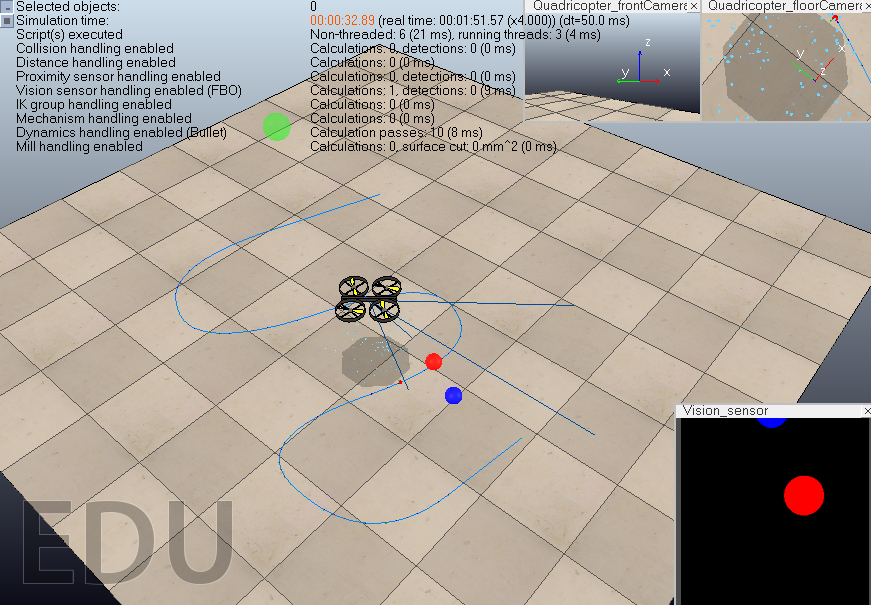
\includegraphics[width=0.4\linewidth]{../Images/c3/sim4_set_up}
	\caption{Objetivos M\'ultiples objetivos}
	\label{fig:sim4_set_up}
\end{figure}

\subsubsection{Test y resultados}

	Como en los apartados anteriores se muestran tres figuras correspondientes a las coordenadas XY original y calculada y la trayectoria 3D (\ref{fig:sim4_redtarget}, \ref{fig:sim4_bluetarget} y \ref{fig:sim4_3dtraj}). \\
	
	\begin{figure}[hp]
		\centering
		\begin{subfigure}[hp]{0.45\linewidth}
			\centering
			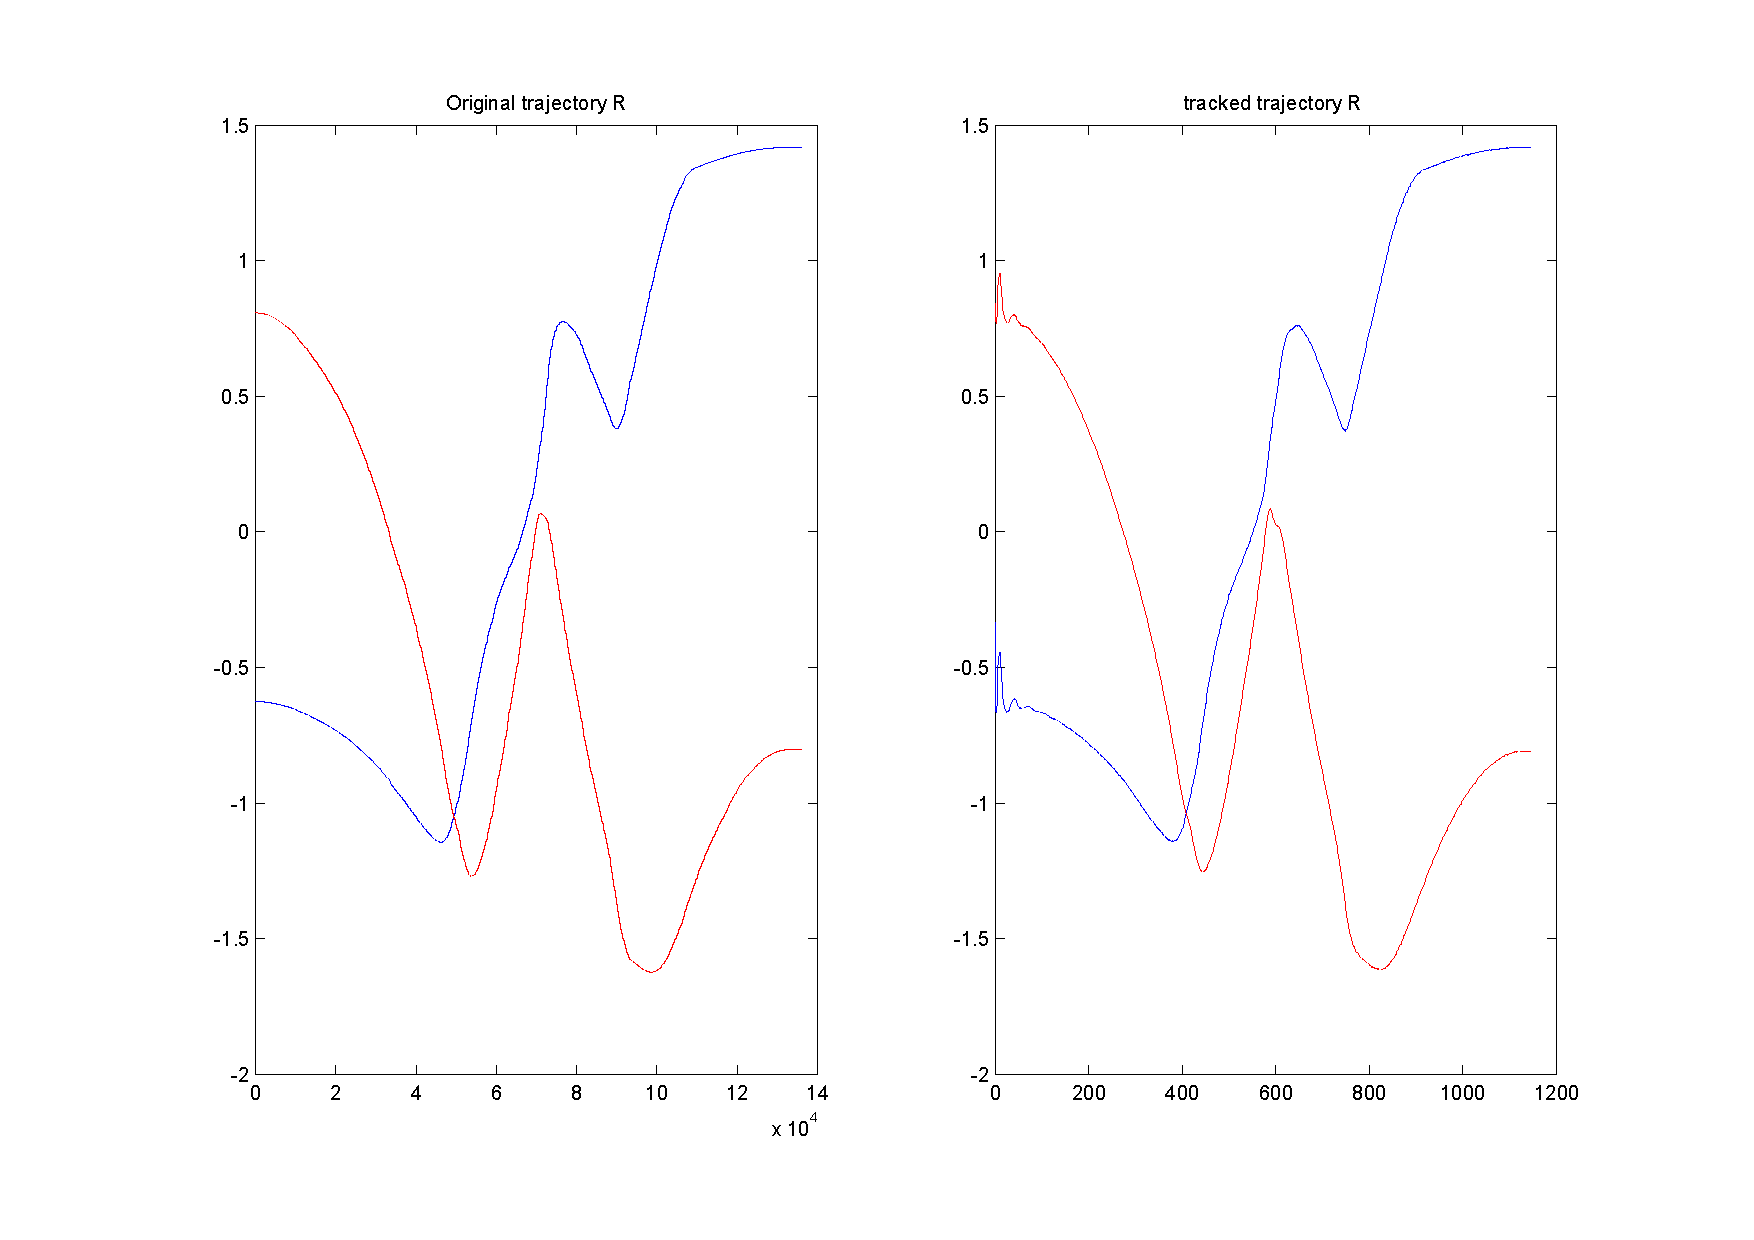
\includegraphics[width=\linewidth]{../Images/c3/sim4_redtarget}
			\caption{Multiple Targets - Red target}
			\label{fig:sim4_redtarget}	
		\end{subfigure}
		~
		\begin{subfigure}[hp]{0.45\linewidth}
			\centering
			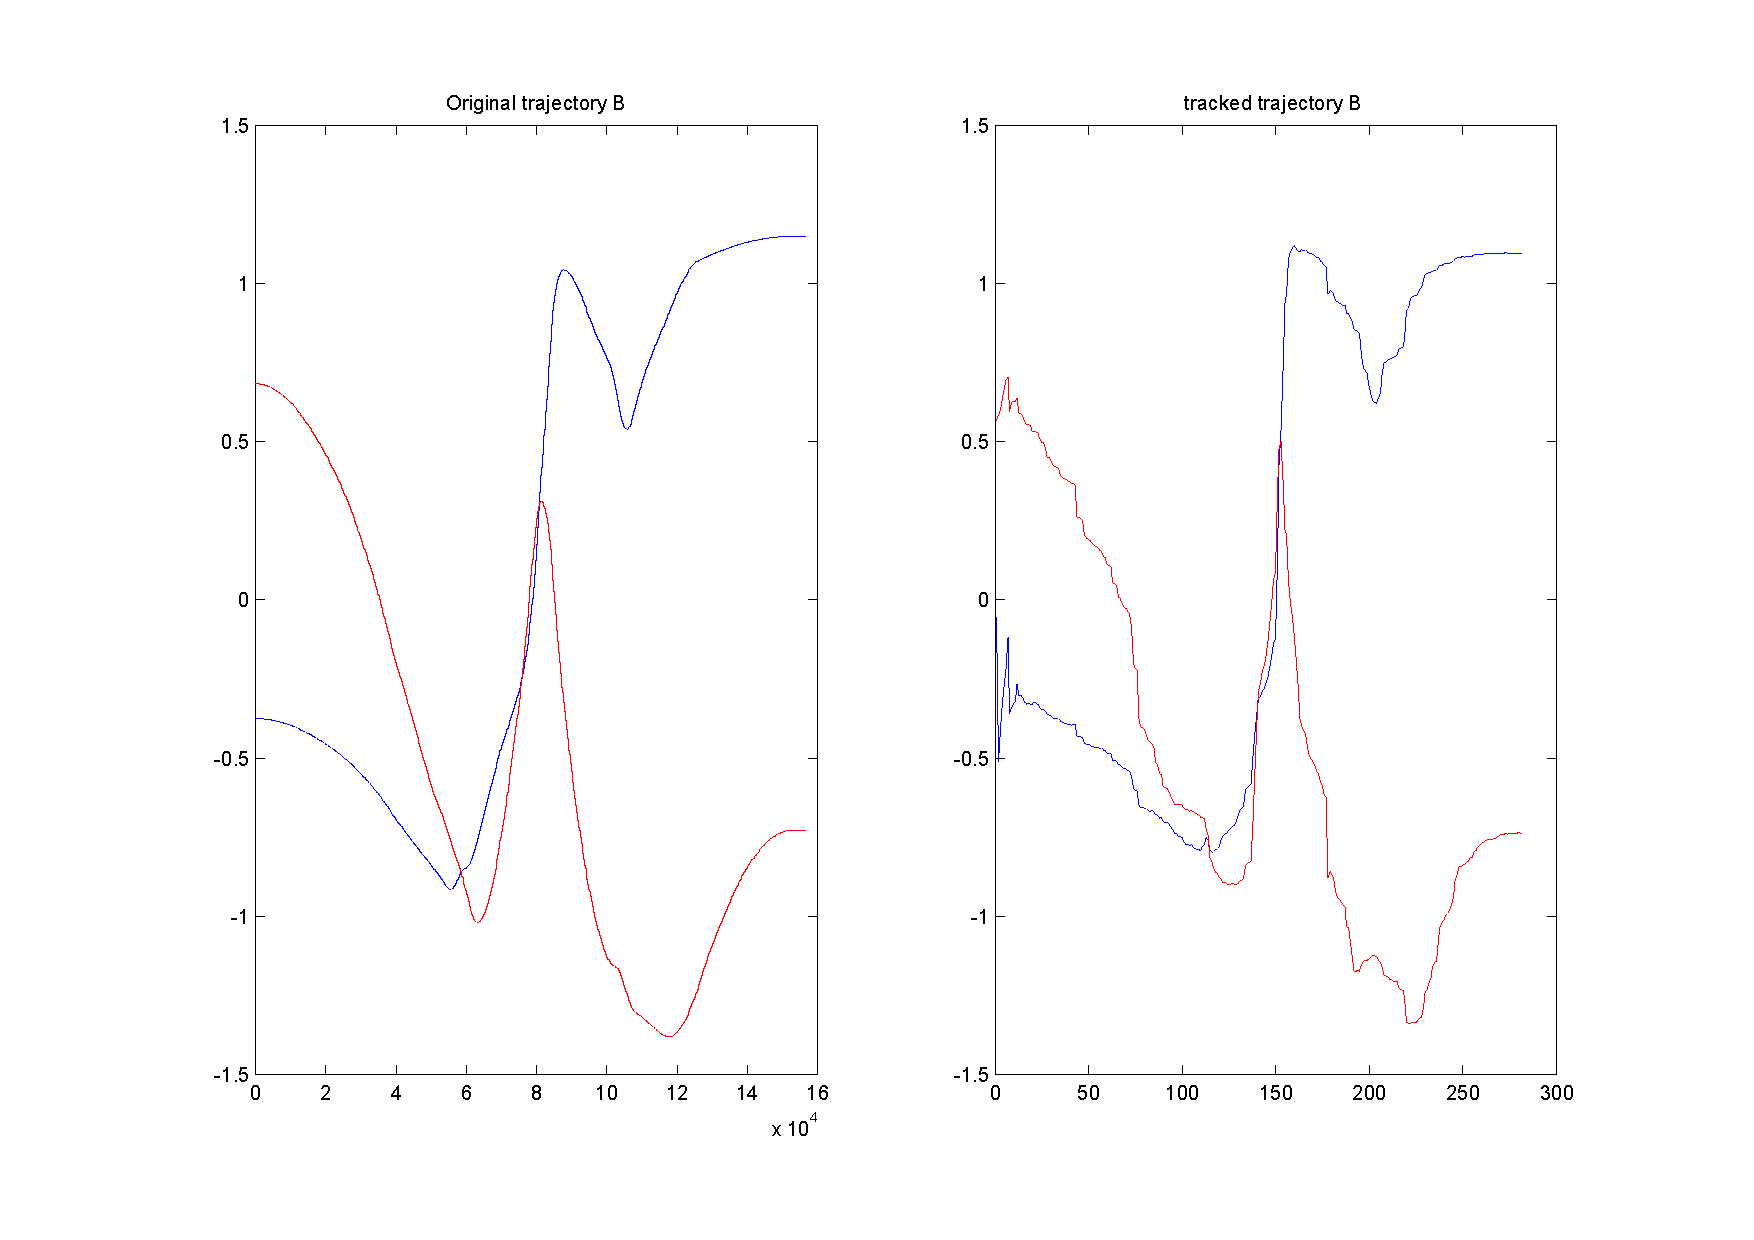
\includegraphics[width=\linewidth]{../Images/c3/sim4_bluetarget}
			\caption{Multiple Targets - Blue target}
			\label{fig:sim4_bluetarget}
		\end{subfigure}
	\end{figure}
	
	El resultado del seguimiento del objeto azul puede parecer erroneo inicialmente, sin embargo es un resultado totalmente coherente ya que este nunca se ve completamente por lo que nunca se obtiene el centro real del mismo \ref{fig:sim4_centroid_objs} y de ah\'i el error en posici\'on. El error m\'aximo en el azul es $\sim$ 15 cm y el medio es $\sim$ 6 cm.



\begin{figure}[hp]
	\centering
	\begin{subfigure}{0.45\linewidth}
		\centering
		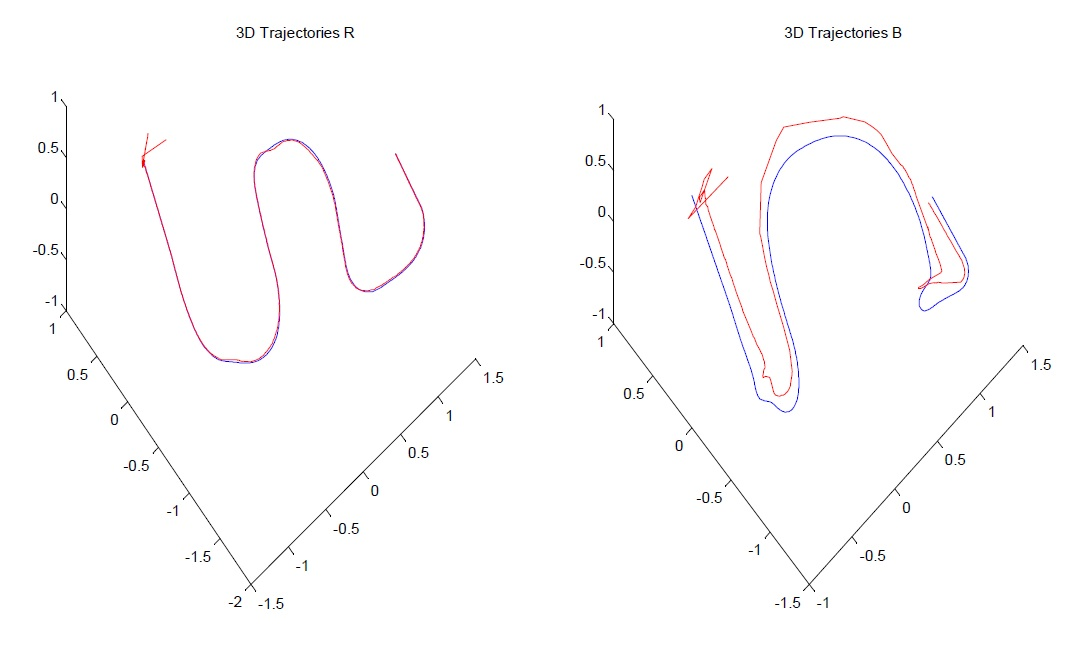
\includegraphics[width=\linewidth]{../Images/c3/sim4_3dtraj}
		\caption{M\'ultiples objetivos - Trayectoria 3D}
		\label{fig:sim4_3dtraj}
	\end{subfigure}
	~
	\begin{subfigure}{0.2\linewidth}
		\centering
		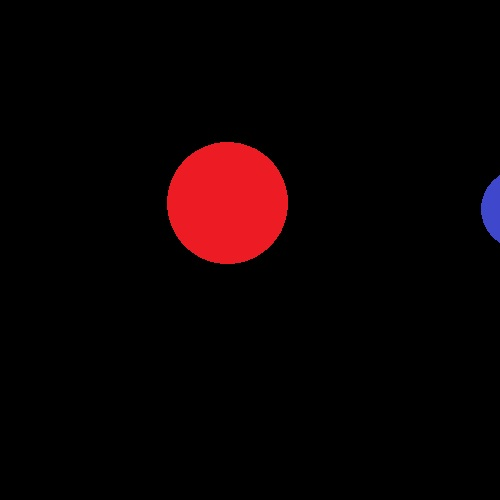
\includegraphics[width=\linewidth]{../Images/c3/sims_two_object_centroid_out}
		\caption{M\'ultiples objetivos - Centroides}
		\label{fig:sim4_centroid_objs}
	\end{subfigure}
\end{figure}

%----------------------------------------------------------
% Chapter 5. Real tests
\chapter{Resultados Experimentales}
\section{Implementaci\'on del Software}

	En esta secci\'on se usaran los datasets obtenidos en unos experimentos realizados en el testbed del CATEC. Para esto se desarrollaron unas aplicaciones para ser ejecutadas dentro de los ordenadores de abordo de los UAVs, mientras que la aplicaci\'on de la estaci\'on de tierra se mantuvo intacta gracias a la capa de abstracci\'on. \ref{fig:Interfaces}
	
	\begin{figure}[th]
		\centering
		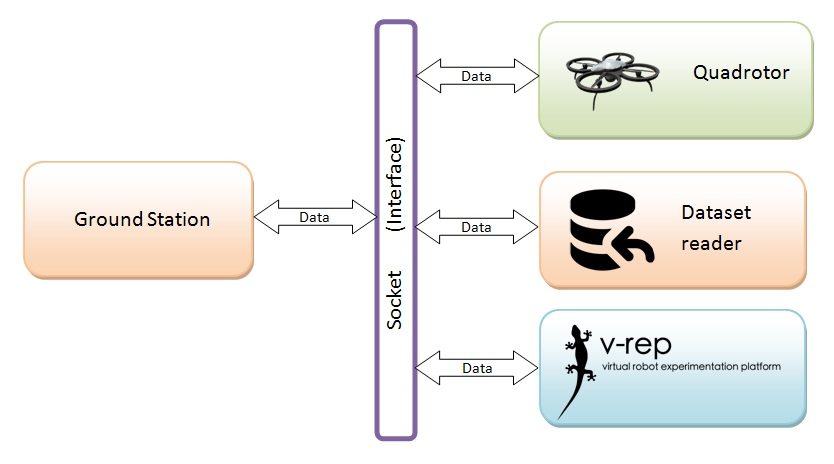
\includegraphics[width=\linewidth]{../Images/c4/Interfaces}
		\caption{Interfaz de comunicaci\'on}
		\label{fig:Interfaces}
	\end{figure}

	

\section{Resultados}
\subsection{Introduction}
	\begin{figure}[h]
		\centering
		\begin{subfigure}{0.49\linewidth}
			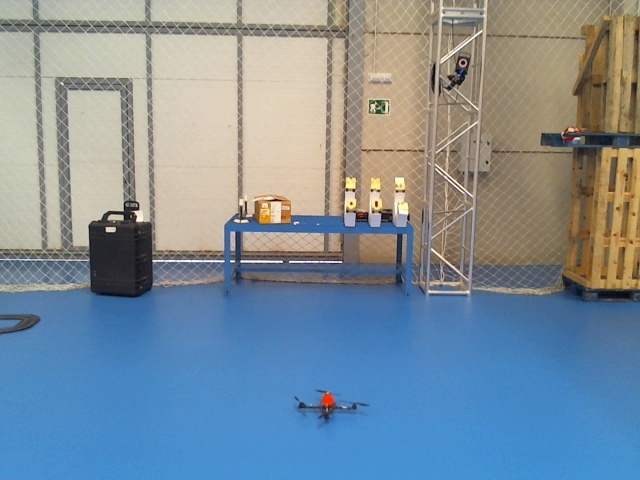
\includegraphics[width=\linewidth]{../Images/c4/image_ori}
			\caption{Original Image}
			\label{fig:image_ori}
		\end{subfigure}
		%--------------------------------------------------------------------
		\begin{subfigure}{0.49\linewidth}
			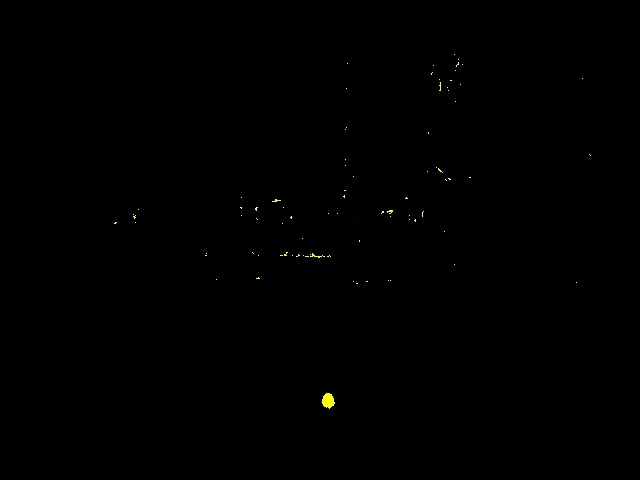
\includegraphics[width=\linewidth]{../Images/c4/image_seg}
			\caption{Segmented Image}
			\label{fig:image_seg}
		\end{subfigure}
		\caption{Images to and from algorithm}
		\label{fig:frames_PC}
	\end{figure}

	La figura: \ref{fig:frames_PC} muestra una imagen del dataset capturada por las c\'amaras de los quadqrotors y el resultado de la segmentaci\'on por color. Sin embargo, a diferencia de las simulaciones en esta hay m\'ultiples objetos pequeños que tienen que ser cribados con un filtro de color y de tama\~no.

\subsection{Test en el PC}
	Caracter\'isticas del sistema:
	\begin{itemize}
		\item{Resoluci\'on de las im\'agenes: 640x480}
		\item{Intel core i7 2.20 GHz. Uso del procesador 7-10\%}
		\item{6 GB of RAM. Uso de la memoria $\sim$ 5000-7000 KB}
	\end{itemize}
	
	\subsubsection{Algoritmo de seguimiento terrestre}
	
	Los datasets fueron grabados en est\'ereo. Sin embargo, las primeras pruebas fueron con los objetivos en tierra por lo que usando la informaci\'ion de una sola de las c\'amaras puede probarse el algoritmo. La siguiente tabla muestra unos estad\'isticos del algoritmo: \\
	
	{
	\centering
		\begin{tabular}{|c|c|c|c|c||c|}
		\hline  					&  Open Image	&  RGB to HSV 	& Segmentation 	& EKF step  & Complete \\ 
		\hline  \textbf{time (ms)}	& 0.0085 		& 0.0015 		& 0.0100 		& 0.0001 	& 0.0231 	\\ 
		\hline  \textbf{fps (1/s)}	&  118			&  645			&  100			& 13936 	& 43 		\\ 
		\hline 
		\end{tabular} 
	}
	\newline

	{
	\label{Reference_fps_table}
	En este caso se hizo una prueba del algoritmo ejecut\'andose de forma secuencial por lo que puede aumentarse la velocidad del mismo paralelizando los procesos en diferentes threads. En la siguiente secci\'on se mostrar\'an los resultados dentro de los ordenadores de abordo con el algoritmo en paralelo. \ref{test_with_odroid_and_GT}
	}
	
	Las siguientes gr\'aficas muestran los resultados de las trayectorias \ref{fig:trajectories_PC} y los errores de estimaci\'on   \ref{fig:errors_PC}. Los errores est\'an acotados superiormente por $0.2 m$.
	
	\begin{figure}[hp]
		\centering
		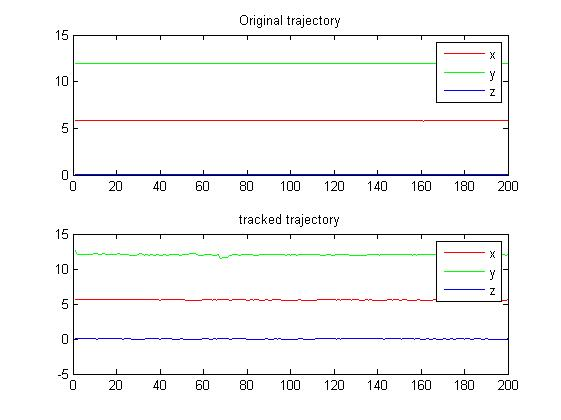
\includegraphics[width=0.75\linewidth]{../Images/c4/trajs}
		\caption{Ejecuci\'on en pc - Trayectorias original y Calculadas.}
		\label{fig:trajectories_PC}
	\end{figure}
	
	\begin{figure}[hp]
		\centering
		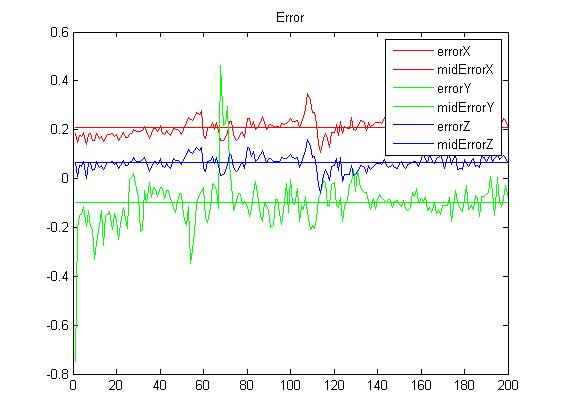
\includegraphics[width=0.5\linewidth]{../Images/c4/errors}
		\caption{Ejecuci\'on en pc - Errores}
		\label{fig:errors_PC}
	\end{figure}
	
	\newpage
	
	%\begin{figure}[ht]
	%	\centering
	%	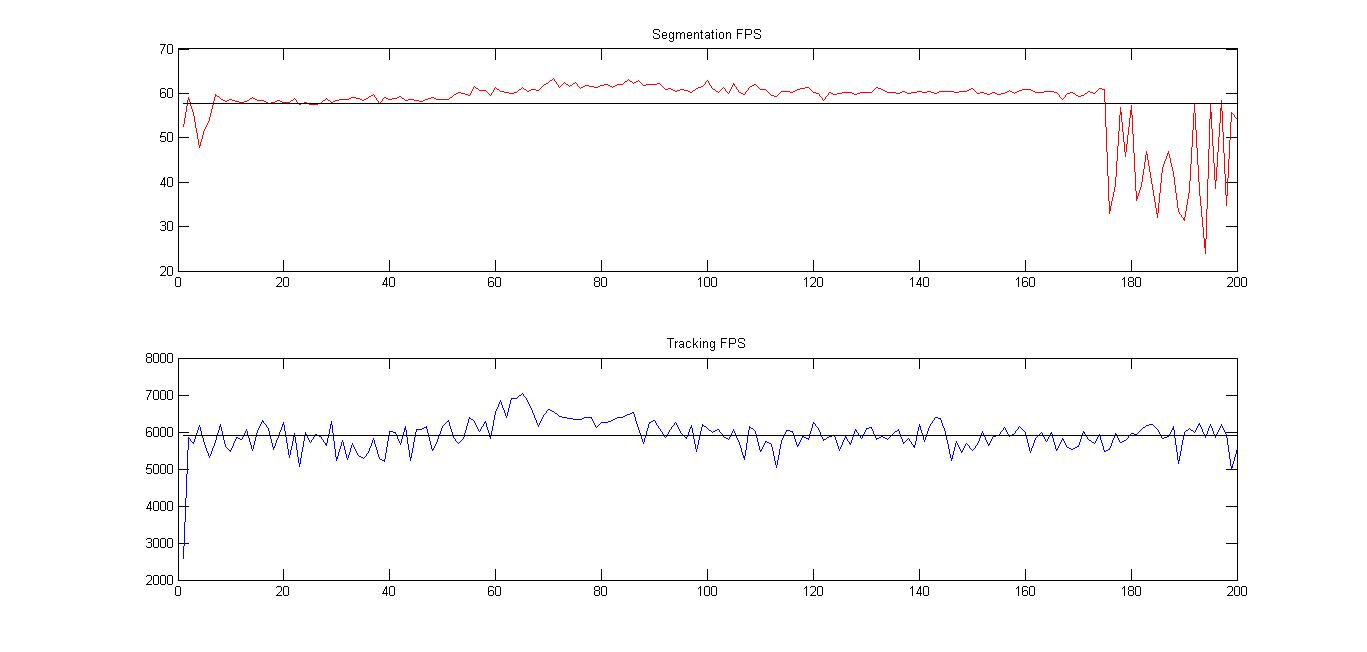
\includegraphics[width=\linewidth]{../Images/c4/fps}
	%	\caption{}
	%	\label{fig:fps_PC}
	%\end{figure}
		
	\subsubsection{Algoritmo de seguimiento est\'ereo}
	
	En este caso se usa la informaci\on de ambas c\'amaras para la estimaci\'on de posici\'on: \\
		
	{                
	\centering
		\begin{tabular}{|c|c|c|c|c||c|}
		\hline  					&  Open Image	&  RGB to HSV 	& Segmentation 	& EKF step  & Complete \\ 
		\hline  \textbf{time (ms)}	&	0.0222		& 	0.0031 		&  	0.0157		&  	0.0001 	&  0.0429		\\ 
		\hline  \textbf{fps (1/s)}	& 	45 			& 	321.5 		& 	63.8 		& 9785.5	&  23.3		\\ 
		\hline 
		\end{tabular} 
	}
	\newline
	
	Esta tabla tiene la misma notaci\'on que la tabla anterior \ref{Reference_fps_table}.
	
	Final mente estas im\'agenes muestran las posiciones originales y calculadas del objetivo \ref{fig:trajectories_stereo_PC} y el error entre ellas \ref{fig:errors_stereo_PC}.
	
	\begin{figure}[hp]
		\centering
		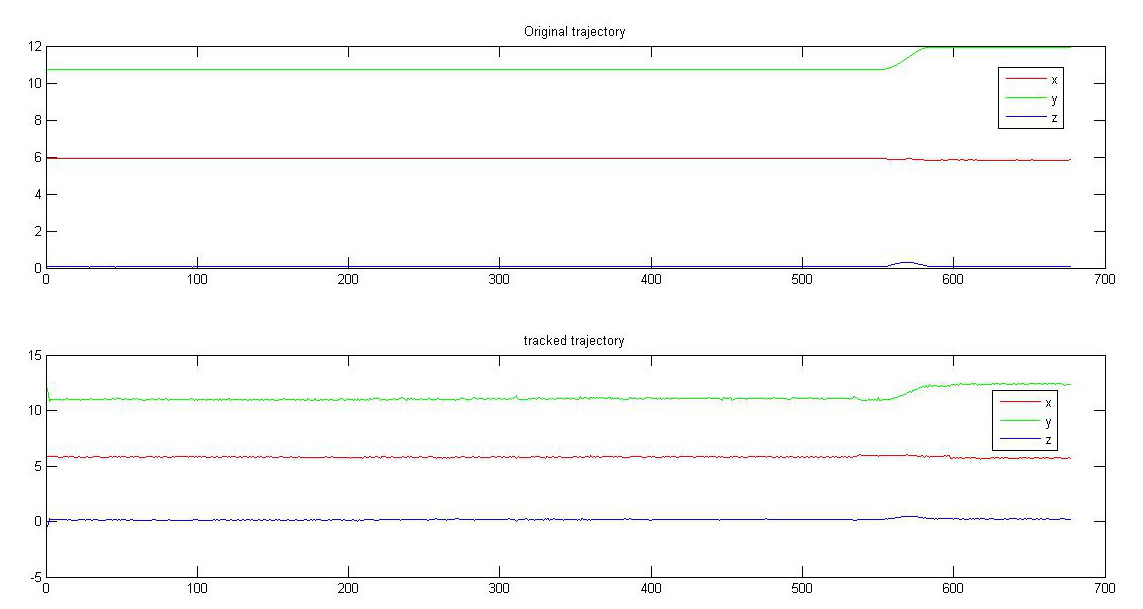
\includegraphics[width=\linewidth]{../Images/c4/trajs_stereo}
		\caption{Algoritmo de seguimiento est\'ereo - Trayectorias original y calculada}
		\label{fig:trajectories_stereo_PC}
	\end{figure}
	
	\begin{figure}[htp]
		\centering
		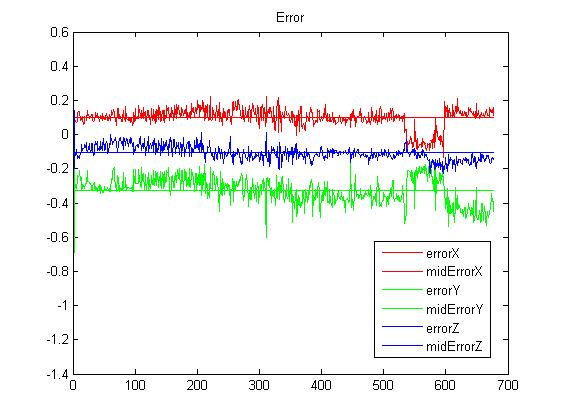
\includegraphics[width=0.7\linewidth]{../Images/c4/errors_stereo}
		\caption{Algoritmo de seguimiento est\'ereo - Errores}
		\label{fig:errors_stereo_PC}
	\end{figure}	
	
	\newpage
	
\subsection{Test en el ordenador de abordo}
	\label{test_with_odroid_and_GT}
	
	\begin{wrapfigure}{r}{0.5\linewidth}
		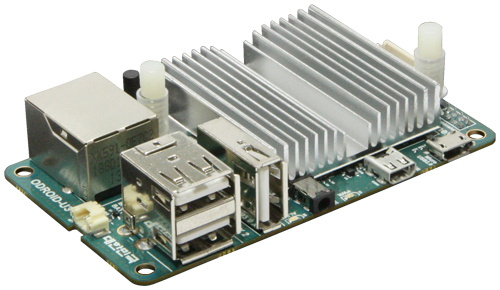
\includegraphics[width=\linewidth]{../Images/c4/odroidu3}
		\caption{Hardkernel Odroid u3}
		\label{fig:odroidu3}
	\end{wrapfigure}
		
	Para estos test se us\'o el esquema de software descrito en secciones anteriores para la estaci\'on en tierra \ref{fig:GroundStation} y para el quadrotor \ref{fig:Quadsoftware}, conectados a trav\'es de la red. La siguiente lista muestra las caracter\'isticas generales del ordenador de abordo (Odroid U3 de Hardkernel)
	
	\begin{itemize}
		\item 1.7GHz Quad-Core processor 
		\item 2GB RAM
		\item GPU ARM Mali-400 Quad Core 440MHz  
	\end{itemize}
	
	\subsubsection{Algoritmo de seguimiento terrestre}
	
	La siguiente tabla muestra los tiempos de ejecuci\'on de cada ciclo de cada hilo del quadrotor:
	% 666 TODO: quitar el filtro de media del tratamiento que ralentiza mucho
	\newline
	\newline
	{
	\centering
		\begin{tabular}{|c|c|c|c|c|c|}
		\hline  					&  Open Img	&  cp Img 	& Vicon 	& Treat img & Comm  		\\ 
		\hline  \textbf{time (ms)}	& 	0.0154	& 0.0018	&	0.00096	&  	 0.019	&	0.0001		\\ 
		\hline  \textbf{fps (1/s)}	&  	68		&  63.2		&  10356	&  	51.23	&	12022		\\ 
		\hline 
		\end{tabular} 
	}
	\newline
	
	Y esta segunda tabla de la estaci\'on en tierra:
	\newline
	
	{
	\centering
		\begin{tabular}{|c|c|c|}
		\hline  					&  comm		&  EKF step	\\
		\hline  \textbf{time (ms)}	& 	0.0001	& 	0.0001	\\
		\hline  \textbf{fps (1/s)}	&  	10567.5	&  	9608.5	\\
		\hline 
		\end{tabular} 
	}
	\newline
	
	El cuello de botella se encuentra de nuevo en la parte de segmentaci\'on ya que es la que requiere m\'as recursos computacionales.
	Finalmente la siguiente figura muestra las trayectorias original y calculadas \ref{fig:arch_trajs}. Cabe mencionar que la cantidad de informaci\'on usada por el algoritmo es menor que la existente, esto se debe al asincronismo de los hilos del sistema. Tal y como ser\'ia en un sistema real, se desechan im\'agenes si estas pueden ser sustituida por unas m\'as recientes El error medio es $\sim$ 0.2m.
	
	\begin{figure}[ph]
		\centering
		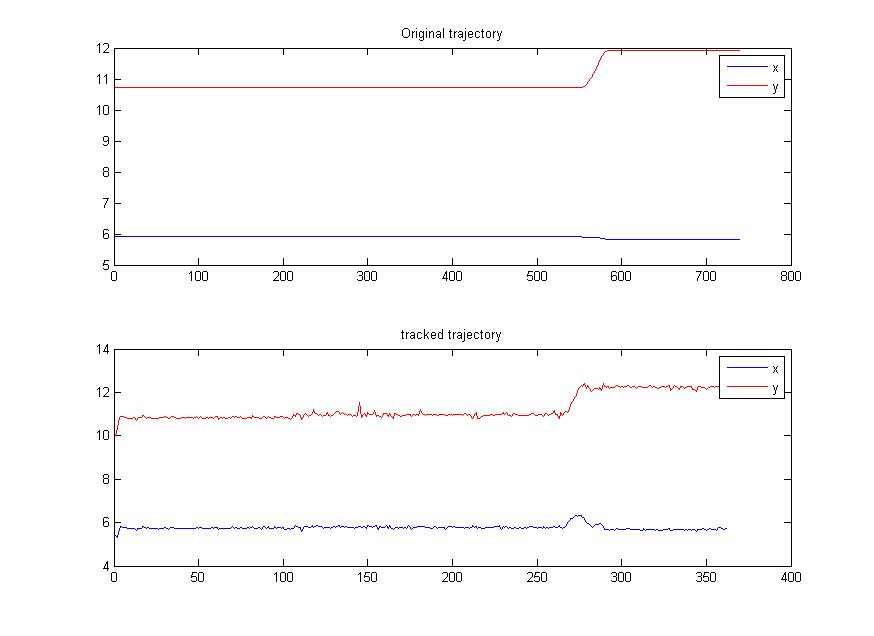
\includegraphics[width=0.5\linewidth]{../Images/c4/arch_trajs}
		\caption{Ejecuci\'on en Odroid - Trayectorias}
		\label{fig:arch_trajs}
	\end{figure}

	
	\subsubsection{Algoritmo de seguimiento est\'ereo}
		En este caso existen dos proveedores de informaci\'on (Dos quadrotors con dos Odroids) que se comunican con la estaci\'on en tierra para el seguimiento del objetivo. La siguiente tabla muestra los tiempos de proceso dentro de la Odroid.
		% 666 TODO: quitar el filtro de media del tratamiento que ralentiza mucho
		\newline
		\newline
		{
		\centering
			\begin{tabular}{|c|c|c|c|c|c|}
			\hline  					&  Open Img	&  cp Img 	& Vicon 	& Treat img & Comm  		\\ 
			\hline  \textbf{time (ms)}	& 	0.0161	& 0.0019	&	0.000098&  	 0.02	&	0.0001		\\ 
			\hline  \textbf{fps (1/s)}	&  	62.11	&  52.631	& 10204.08 	&  49.56	&	986.1	\\ 
			\hline 
			\end{tabular} 
		}
		\newline
		
		Esta segunda tabla muestra los tiempos en la estaci\'on en tierra.
		\newline
		
		{
		\centering
			\begin{tabular}{|c|c|c|}
			\hline  					&  comm		&  EKF step	\\
			\hline  \textbf{time (ms)}	& 	0.0001	& 	0.0001	\\
			\hline  \textbf{fps (1/s)}	&  	10368.5	&   9898.6 	\\
			\hline 
			\end{tabular} 
		}
		\newline
	\begin{figure}[ph]
		\centering
		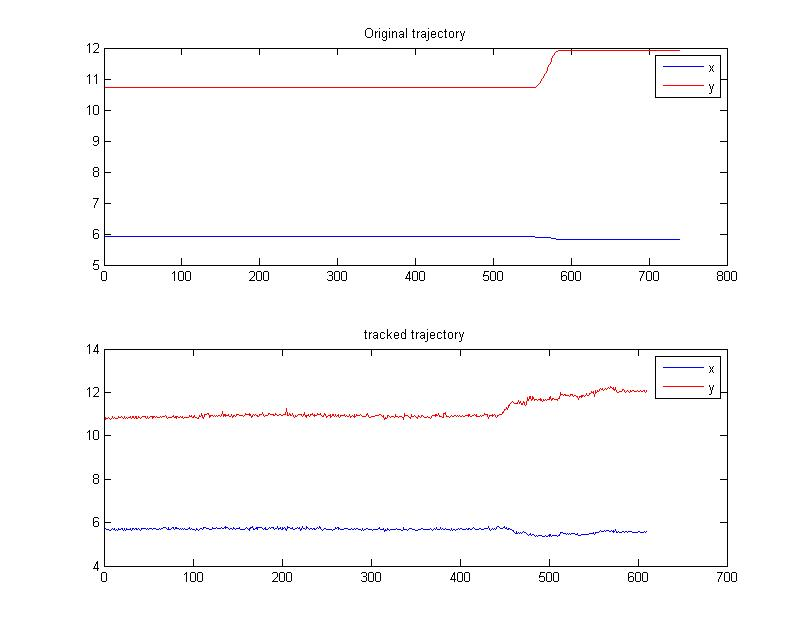
\includegraphics[width=0.7\linewidth]{../Images/c4/arch_trajs_stero}
		\caption{Ejecuci\'on en Odroid - Trayectorias}
		\label{fig:arch_trajs_stero}
	\end{figure}
	
	\begin{figure}[ph]
		\centering
		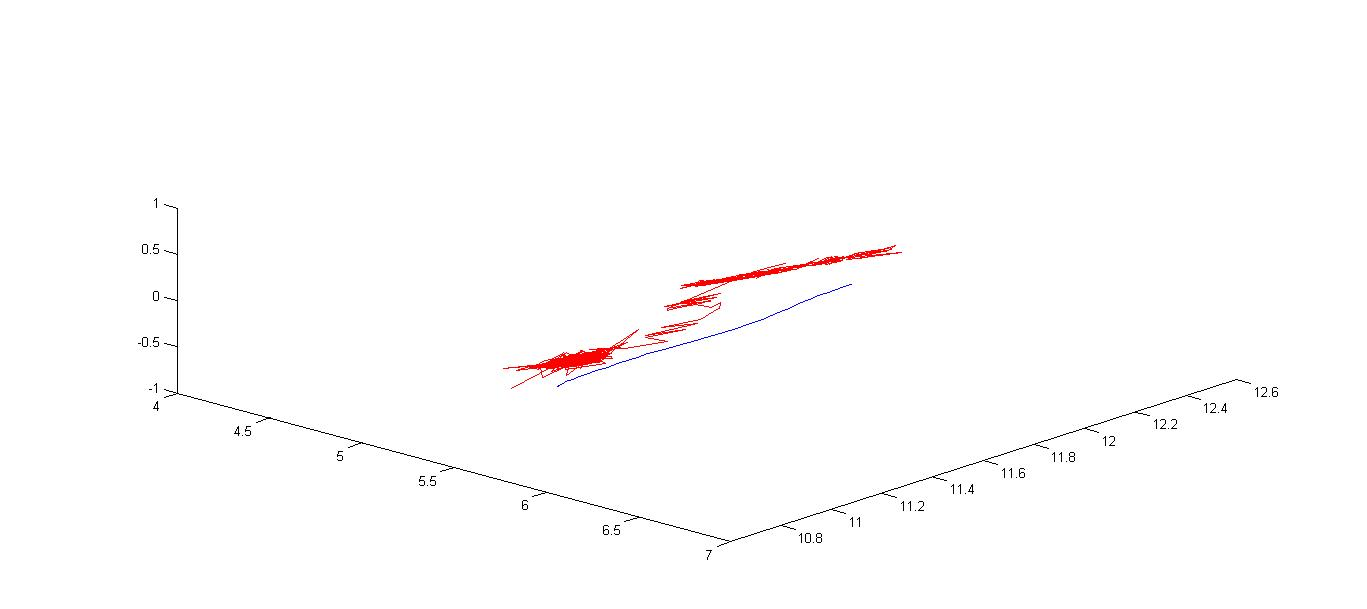
\includegraphics[width=0.6\linewidth]{../Images/c4/arch_3d_trajs_stero}
		\caption{Ejecuci\'on en Odroid - Trayectorias 3D}
		\label{fig:arch_3d_trajs_stero}
	\end{figure}



%----------------------------------------------------------
% Chapter 6. Conclusions
\chapter{Conclusiones} \label{chap:c6_conclusions}
\section{Introducci\'on}
	Resumiendo, este documento muestra un algoritmo de tracking basado en visi\'on para ser usados en UAVs. Este algoritmo es capaz de realizar tracking de m\'ultiples objetos basados en su color. Esta caracter\'istica es una de las principales ventajas del algoritmo frente a otros como CAMSHIFT's \cite{CAMSHIFT_FAST} \cite{CAMSHIFT_ENVIROMENT}. El cuello de botella de los algoritmos de segmentaci\'on es el tiempo de computaci\'on, sin embargo el algoritmo descrito anteriormente permite al ordenador de abordo de los UAVs procesar r\'apidamente las im\'agenes capturadas.
	En paralelo al desarrollo del algoritmo se desarrol\'o una libreria multi-plataforma parar poder hacer un uso r\'apido del c\'odigo. A parte de otras ventajas que conlleva el control de versiones. El ap\'endice \ref{chap:c6_bovil} contiene una breve descripci\'on de la librer\'ia
	% % TODO 666 ADD CITES!!
	
\section{Ramas futuras}	
	\subsection{Color Clustering en paralelo}
	Como ya se ha comentado, el principal cuello de botella es la segmentaci\'on por color. Cada paso del algoritmo comprueba cada p\'ixel de la im\'agen, por lo que se puede reestructurar esta parte del algoritmo con el paradigma de procesamiento paralelo. Usando la unidad de procesamiento gr\'afica (GPU) en vez de la CPU es posible aumentar notablemente la velocidad del proceso \cite{GPU_CPU_performance} \cite{GPU_parallel_image_processing} \cite{GPU_enabled_parrallel}.
		
	\begin{figure}[ph]
		\centering
		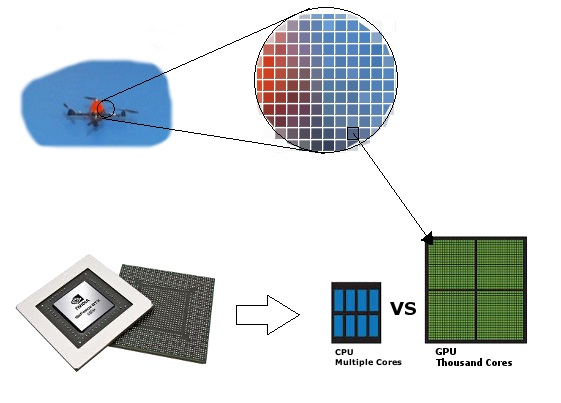
\includegraphics[width=0.7\linewidth]{../Images/c5/gpu}
		\caption{Paralelizaci\'on}
		\label{fig:gpu}
	\end{figure}


	\subsection{Reconocimiento de Formas}
	Hasta ahora, el criterio de selecci\'on de objetivo se realiza por color y tama\~no. Sin embargo esto puede causar problemas cuando existen m\'ultiples posibles objetivos en la escena. El reconocimiento de patrones o formas  \cite{color_shape_object_recogn} \cite{Fast_object_recogn_shape} podr\'ia ser una herramienta muy \'util para esta parte del algoritmo:
	
	\begin{figure}[th]
		\centering
		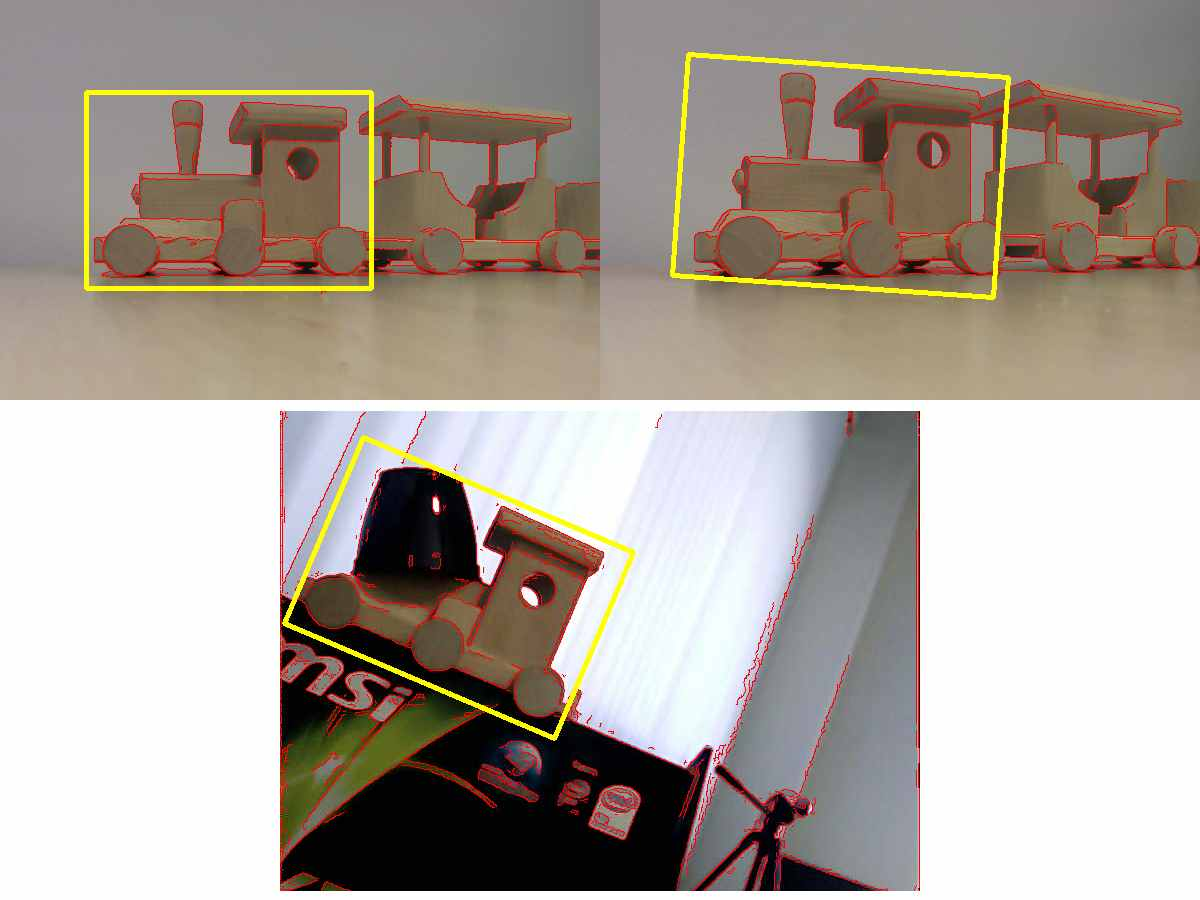
\includegraphics[width=0.6\linewidth]{../Images/c6/shape_recogn}
		\caption{Reconocimiento de Formas}
		\label{fig:shape_recogn}
	\end{figure}
	
	\subsection{Big Data}
	Este t\'ermino se refiere  a la recolecci\'on de grandes cantidades de datos con estructuras diversas y complejas. En este punto resulta complicado procesar esa cantidad de informaci\'on. Plantear una correcta arquitectura para el "Data mining" \cite{Big_data_Ecosystem} \cite{Big_data_mapReduce} puede prevenir al sistema de colapsar en caso de grandes caudales de informaci\'on:
	
	\begin{figure}[th]
		\centering
		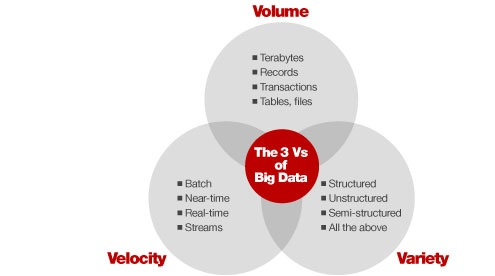
\includegraphics[width=0.7\linewidth]{../Images/c6/big_data}
		\caption{Big Data}
		\label{fig:big_data}
	\end{figure}
	
	


%----------------------------------------------------------
\begin{appendix}
\chapter{BOViL} \label{chap:c6_bovil}
\section{Introduction}
	\begin{wrapfigure}{r}{0.3\textwidth}
		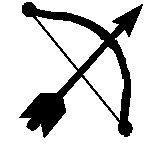
\includegraphics[width=0.3\textwidth]{../Images/c6/BOVIL.jpg}
		\label{fig:bovil}
	\end{wrapfigure}

	% % TODO 666 intro de la web
	The code and the documentation of the library can be found in the website \cite{BOViL}
	
\section{Content}
	The library is divided in to main sections:
	\begin{itemize}
		\item \textit{Core}: This section include some basics that could be helpful in every kind of application and algorithm; as an easy socket implementation, matrix operations, timing, and so on.
		\item \textit{Algorithms}: In this section are implemented a variety of algorithm; as the color clustering used and described in this project and the EKF tracking algorithm for ground and flying targets.
	\end{itemize}
	
	\subsubsection{Core}
		\begin{itemize}
			\item \textit{Communication}: Fast implementation of cross-platform sockets. The use is described on the wiki and accept any kind of UDP and TCP/IP sockets.
			\item \textit{Math}:
				\begin{itemize}
					\item \textit{Matrix}: \textit{Easy to use} matrix implementation.
					\item \textit{Geometrics}: Linear subspace class implementation.
				\end{itemize}
			\item \textit{Time}: Cross-platform time management.
			\item \textit{Types}: Basic types used in the library
		\end{itemize}
		
	\subsubsection{Algorithms}
		\begin{itemize}
			\item \textit{Segmentation}: Implementation of segmentation algorithm. At present, only color-based segmentation is implemented.
			\item \textit{State Estimators}: 
			\begin{itemize}
				\item \textit{ExtendedKalmanFilter}: Basic template of Extended Kalman Filter. It's used to implement easily any kind of EKF overriding the jacobians.
				\item \textit{GroundEKF}: derived class of \textit{ExtendedKalmanFilter} that override its jacobian for ground tracking.
				\item \textit{StereoEKF}: derived class of \textit{ExtendedKalmanFilter} that override its jacobian for stereo tracking.
			\end{itemize}
		\end{itemize}
\end{appendix}

%----------------------------------------------------------
\listoffigures{}

%----------------------------------------------------------
% Bibliography
\begin{thebibliography}{9}
% \bibitem{} \textit{} 

\bibitem{Image_processing_UAV} Ryan Carnie, Rodney Walker and Peter Corke \textit{Image Processing Algorithms for UAV “Sense and Avoid”} 

\bibitem{traffic_surveillance_pergamon} Benjamin Coifmana, David Beymerb, Philip McLauchlanb and Jitendra Malikb\textit{A real-time computer vision system for vehicle tracking and trac surveillance} 

\bibitem{distributed_surveillance} M. Valera and S.A. Velastin \textit{Intelligent distributed surveillance systems} 

\bibitem{vehicle_detection} D.Neelima and Gowtham Mamidisetti \textit{Computer Vision Model for Vehicle Detection in Traffic Surveillance} 

\bibitem{Kinect_intro} Jungong Han, Ling Shao, Dong Xu and Jamie Shotton \textit{Enhanced Computer Vision with Microsoft Kinect Sensor: A Review.} 

\bibitem{Coop_Surv_aerial_JJ} Jose Joaquin Acevedo, Bego\~na Arrue, Ivan Maza and Anibal Ollero \textit{Cooperative large area surveillance with a team of aerial mobile robots for long endurance missions}


\bibitem{Consensus_reaching_Xiao} Xiaojun Geng. \textit{ Consensus-reaching of multiple robots with fewer interactions }. In $Computer Science and Information Engineering$, 2009 WRI World Congress on, volume 5, pages 249 - 253, 31 2009-april 2 2009.

\bibitem{Adaptative_tast_Meuth} R.J. Meuth, E.W. Saad, D.C. Wunsch, and J. Vian. \textit{Adaptive task allocation for search area coverage} . In $Technologies for Practical Robot Applications$, 2009.TePRA 2009. IEEE International Conference on, pages 67-74, nov. 2009.

\bibitem{distributed_architecture_Ivan_Maza} Ivan Maza, Fernando Caballero, Jesus Capitan, J.R. Martinez de Dios and Anibal Ollero \textit{A Distributed Architecture for a Robotic Platform with Aerial Sensor Transportation and Self-Deployment Capabilities} Robotics, Vision and Control Group. Universidad de Sevilla.

\bibitem{descentralized_task_UAV} Edison Pignaton de Freitas, Tales Heimfarth, Armando Morado Ferreira, Carlos Eduardo Pereira, Flavio Rech Wagner and Tony Larsson \textit{Decentralized Task Distribution among Cooperative UAVs in Surveillance Systems Applications}

\bibitem{shape_using_shape_context} Serger Belongie, Jitendra Malik, Jan Puzicha \textit{Shape Matching and Object Recognition Using Shape Context} IEEE Transaction on pattern analysis and machine intelligence. April 2002

\bibitem{CAMSHIFT_FAST} David Exner, Erich Bruns, Daniel Kurz, Anselm Grundhofer and Oliver Bimber  \textit{Fast and Robust CAMShift Tracking}

\bibitem{CAMSHIFT_ENVIROMENT} Lae-Kyoung Lee, Su-Yong An, and Se-Young Oh  \textit{ Robust Visual Object Tracking with Extended CAMShift in Complex Environments}
 
\bibitem{Vehicle_recog_markov} Tian-min Deng, Yi-ming Shao, Min Li, and Li Lin \textit{Vehicle Recognition Based on Gabor Wavelets Transform and Hidden Markov Model} American Society of Civil Engineers. 2007
 
\bibitem{realtime_signal_recon_shape_color} Alberto Broggi, Pietro Cerri, Paolo Medici, Pier Paolo Porta and Guido Ghisio  \textit{Real Time Road Signs Recognition} IEEE Intelligent Vehicles Symposium Istanbul, Turkey, June 13-15, 2007

\bibitem{signal_recogn_shape_color} Claw Bahlmann, Ying Zhu, Visvanathan Ramesh, Martin Pellkofert and Thorstea Koehled  \textit{A System for Traffic Sign Detection, Tracking, and 	Recognition Using Color, Shape, and Motion Information}

\bibitem{Robust_RT_tracking_color_face_Darrell} Darrell, T., Gordon, G., Woodfill, J., Baker, H., and Harville, M. \textit{Robust real-time people tracking in open environments using integrated stereo, color, and face detection}. 3rd IEEE workshop on visual surveillance, India, 1998, pp. 26–33.

\bibitem{JamesBruce_CMU_SEG} James Bruce, Tucker Balch, Manuela Veloso  \textit{Fast and Inexpensive Color Image Segmentation for Interactive Robots.} . IROS2000. School of Computer Science Carnegie Mellon University

\bibitem{GabrielTerejanu_EKF} Gabriel A. Terejanu \textit{Extended Kalman Filter Tutorial} . IROS2000. Department of Computer Science and Engineering, University at Buffalo

\bibitem{fast_segmentation_Mitra} L. Lucchese and S.K. Mitra \textit{An Algorithm for Fast Segmentation of Color Images}

\bibitem{fuzzy_segmentation} Hoel Le Capitaine and Carl Frélicot \textit{A fast fuzzy c-means algorithm for color image segmentation}

\bibitem{camera_models}  Leow Wee Kheng \textit{Camera Models and Imaging}

\bibitem{GPU_CPU_performance} Shuichi Asano, Tsutomu Maruyama and Yoshiki Yamaguchi \textit{Performance Comparison of FPGA, GPU and CPU in image processing}

\bibitem{GPU_parallel_image_processing} Nan Zhang, Jian-li Wang and Yun-shan Chen  \textit{Image Parallel Processing Based on GPU }

\bibitem{GPU_enabled_parrallel} Barry Trager, Chai Wah Wu, Mikel Stanich, Kartheek Chandu  \textit{GPU-enabled parallel processing for image halftoning applications}

\bibitem{color_shape_object_recogn}  Aristeidis Diplaros, Theo Gevers and Ioannis Patras \textit{Combining Color and Shape Information for Illumination-Viewpoint Invariant Object Recognition}

\bibitem{Fast_object_recogn_shape} Wei Wang, Lili Chen, Dongming Chen, Shile Li and Kolja Kuhnlenz  \textit{Fast Object Recognition and 6D Pose Estimation Using ViewPoint Oriented Color-Shape Histogram}

\bibitem{task_allocation} José Joaquín Acevedo B\'añez  \textit{Cooperation of multiple heterogeneous aerial robots in surveillance missions}

\bibitem{Multirate_sampled_uav}  Camilo Ossa-Gomez and Luis Rodrigues \textit{Multi-Rate Sampled-Data Control of a Fly-by-wireless Autonomous Quadrotor Helicopter}

\bibitem{multi_uav_path_planning} Hui Bai, Shihuang Shao and Hongyu Wang \textit{A VTOL quadrotor platform for Multi-UAV path planning}

\bibitem{Big_data_Ecosystem} Yuri Demchenko, Cees de Laat and Peter Membrey \textit{Defining Architecture Components of the Big Data Ecosystem }

\bibitem{Big_data_mapReduce} Shweta Pandey  and Dr.Vrinda Tokekar \textit{Prominence of MapReduce in BIG DATA Processing}

\bibitem{}   \textit{}

\bibitem{SocketWiki} \textit{Network Socket} \url{http://en.wikipedia.org/wiki/Network_socket}

\bibitem{BOViL} \textit{Bardo's Open Vision Library} \url{https://github.com/Bardo91/BOVIL/wiki}

\bibitem{TCPIP} \textit{TCP/IP Protocol}  \url{http://en.wikipedia.org/wiki/TCP/IP_model}

\bibitem{Cloud_computing} T-Systems Enterprise Services GmbH 2008\textit{White Paper Cloud Computing. T - Systems} 

\bibitem{CATEC} \textit {CATEC's Tesbed} \url{http://www.catec.aero/}

\end{thebibliography}

%----------------------------------------------------------
% Ending
\backmatter

\chapter{Afterword}

\end{document}
